\documentclass[parindent=0pt,11pt,a4paper]{article}

% basic packages
\usepackage{float}
\usepackage{polski}
\usepackage{fullpage}
\usepackage{graphicx}
\usepackage[utf8x]{inputenc}
\usepackage{longtable}

% numbering the paragraphs
\setcounter{secnumdepth}{5}

% links
\usepackage{url}
\usepackage[hidelinks]{hyperref}

\begin{document}

\begin{titlepage}
  \begin{center}

    \textsc{\Large Politechnika Warszawska}\\[0.1cm]
    \small Wydział Elektroniki i Technik Informacyjnych
    \vfill

    \textsc{\small Architektura i Projektowanie Systemów Informacyjnych}\\[0.1cm]
    \Huge System zarządzania wydatkami domowymi\\[1.5cm]
    \small Projekt -- Iteracja 2\\[2.5cm]

    \vfill

    \begin{minipage}{0.4\textwidth}
      \begin{flushleft} \large
        \emph{Zespół:}\\[0.1cm]
        Jakub \textsc{Borowski}\\
        Wojciech \textsc{Matuszewski}\\
        Maciej \textsc{Suchecki}\\
        Daniel \textsc{Waślicki}\\
      \end{flushleft}
    \end{minipage}
    \begin{minipage}{0.4\textwidth}
      \begin{flushright} \large
        \emph{Prowadzący:}\\[0.1cm]
        dr~inż. Andrzej \textsc{Ciemski}\\[1cm]
      \end{flushright}
    \end{minipage}

    \vfill
    {\large \today}

  \end{center}
\end{titlepage}

\newpage
\tableofcontents

\newpage
\section{Wstęp}

Celem utworzenia niniejszego dokumentu jest opisanie oraz zaprezentowanie realizacji projektu systemu informatycznego dla firmy \emph{Money Solutions sp.~z~o.o.} Wspomniana firma jest liderem w~branży doradztwa finansowego, skierowanego głównie do~klientów prywatnych. Z~racji na~rosnące zapotrzebowanie rynkowe na~usługi doradcze w~zakresie prowadzenia budżetu domowego, firma \emph{Money Solutions} zdecydowała się na~zamówienie systemu pozwalającego na~zarządzanie finansami domowymi, który będzie odpłatnie udostępniany jej klientom.\\

Zabieg taki pozwoli na~transfer niektórych obowiązków związanych ze~zbieraniem informacji nt.~budżetu domowego klientów do~nich samych. Dzięki temu każdy z~pracowników firmy \emph{Money Solutions} będzie mógł świadczyć swoje usługi większej liczbie klientów, jednocześnie zwiększając zyski firmy. Ponadto, wspomniany system będzie mógł być również oferowany jako osobna usługa, bez wspomnianego wcześniej doradztwa pracowników firmy.\\

Realizacja systemu została zlecona przez firmę \emph{Money Solutions~sp.~z~o.o.}, zwaną dalej Zleceniodawcą, firmie \emph{Four Developers~sp.~z~o.o.}, zwanej dalej Zleceniobiorcą, autorem tego dokumentu. System powinien spełnić wszystkie wymagania biznesowe postawione przed Zleceniobiorcą, które zostaną opisane w~dalszej części dokumentu. Zleceniobiorca zobowiązuje się do~wykonania wszystkich opisanych w~dokumencie części systemu, uruchomienie jej w~siedzibie firmy \emph{Money Solutions} oraz utrzymania systemu po wdrożeniu (z~czym wiąże się miesięczna opłata). 

\newpage
\section{Zakres realizacji}

% TODO

\newpage
\section{Wymagania}
W tej sekcji znajduje się lista wymagań, jakie spełniać powinien budowany system. Podane są~one z~podziałem na~dwie kategorie. Pierwsza to wymagania funkcjonalne -- określające funkcjonalności systemu oraz sposoby ich użycia. Natomiast druga to~wymagania niefunkcjonalne, które opisują ilościowe i~jakościowe warunki działania systemu.

\subsection{Wymagania funkcjonalne}
\subsubsection{Użytkownicy}
Wymagania funkcjonalne dotyczące zarządzaniem użytkownikami w~systemie.
\begin{itemize}
  \item logowanie do aplikacji,
  \item wyświetlanie listy użytkowników,
  \item dodawanie nowego użytkownika,
  \item edycja danych użytkownika,
  \item usunięcie użytkownika.
\end{itemize}

\subsubsection{Konta}
Wymagania funkcjonalne dotyczące zarządzaniem kontami pieniężnymi w~systemie.
\begin{itemize}
  \item wyświetlanie listy kont,
  \item dodawanie nowego konta,
  \item edycja danych konta,
  \item usunięcie konta.
\end{itemize}

\subsubsection{Transakcje}
Wymagania funkcjonalne dotyczące zarządzaniem transakcjami w~systemie.
\begin{itemize}
  \item wyświetlanie listy transakcji,
  \item dodawanie nowej transakcji,
  \item edycja danych transakcji,
  \item usunięcie transakcji.
\end{itemize}

\subsubsection{Budżet}
Wymagania funkcjonalne dotyczące zarządzaniem budżetami w~systemie.
\begin{itemize}
  \item wyświetlenie budżetów ustawionych w~systemie,
  \item ustawienie budżetu dla określonego użytkownika,
  \item modyfikacja budżetu sumarycznego dla wszystkich użytkowników,
  \item modyfikacja budżetu określonego użytkownika,
  \item usunięcie budżetu określonego użytkownika.
\end{itemize}

\subsubsection{Raporty}
Wymagania funkcjonalne dotyczące generowania raportów w~systemie.
\begin{itemize}
  \item konfiguracja raportu,
  \item wyświetlanie raportu,
  \item zapisywanie raportu do~pliku.
\end{itemize}

\subsubsection{Opis przypadków użycia -- użytkownicy}

\begin{figure}[H]
  \centering
  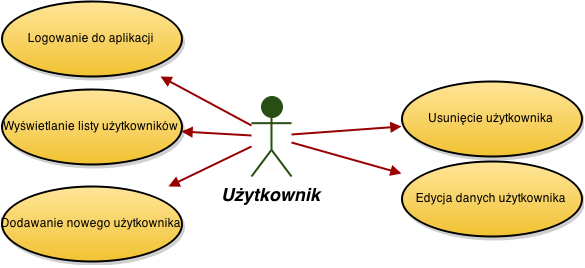
\includegraphics[width=0.7\textwidth]{images/przypadki_uzytkownik.png}
  \caption{Diagram przypadków użycia związanych z~kontami użytkowników.}
\end{figure}

\paragraph{Dodawanie nowego użytkownika\newline}
\label{par:register}

\textit{Opis słowny} -- niniejszy przypadek użycia umożliwia użytkownikowi stworzenie konta, poprzez które będzie miał
on dostęp do systemu.

\begin{longtable}{|p{5cm}|p{8cm}|}
  \hline \textbf{Aktor} & Użytkownik \\ \hline
  \textbf{Warunki początkowe} & Użytkownik nie jest zarejestrowany \\ \hline
  \textbf{Opis przebiegu interakcji} & Wybór strony z~rejestracją, wprowadzenie danych, kliknięcie przycisku,
  zatwierdzenie \\ \hline
  \textbf{Sytuacje wyjątkowe} & Niepoprawnie wprowadzone dane \\ \hline
  \textbf{Warunki końcowe} & Nowy użytkownik w~systemie \\ \hline
\end{longtable}

\noindent \textit{Scenariusz główny:}
\begin{enumerate}
  \item Użytkownik otwiera stronę ,,Logowanie/Rejestracja''.
  \item Użytkownik wybiera opcję ,,Rejestracja'' i~wprowadza niezbędne dane.
  \item Użytkownik naciska przycisk ,,Zarejestruj''.
  \item Aplikacja sprawdza wprowadzone dane.
  \item Jeżeli nie wystąpiły żadne błędy, system wysyła aktywacyjną wiadomość e-mail na adres wprowadzony przez użytkownika i~informuje go, aby go odebrał.
  \item Użytkownik otwiera wiadomość i~klika w~link aktywacyjny.
  \item Aplikacja rejestruje nowego użytkownika i~przekierowuje go do strony logowania.
\end{enumerate}

\noindent \textit{Scenariusz alternatywny -- niepoprawne dane:}
\begin{enumerate}
  \item[1-4.] Jak w~scenariuszu głównym.
  \item[5.] System wyświetla informacje o~wykrytym błędzie.
  \item[6.] Użytkownik poprawia wprowadzone dane i~naciska przycisk ,,Zarejestruj''.
  \item[7.] Powrót do kroku 4.~ze scenariusza głównego.
\end{enumerate}

\begin{figure}[H]
  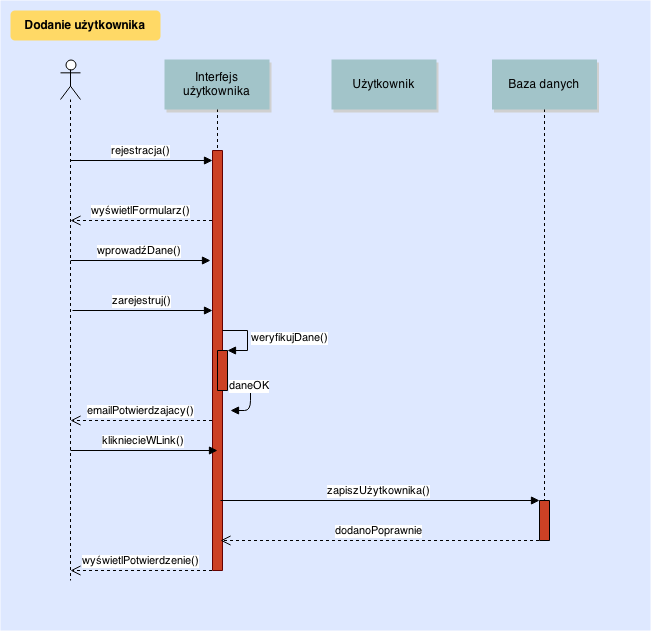
\includegraphics[width=\textwidth]{images/dodaj_uzytkownika.png}
  \caption{Diagram sekwencji dla przypadku użycia~\ref{par:register}~--~Dodawanie nowego użytkownika (scenariusz główny)}
\end{figure}

\newpage
\paragraph{Logowanie do~aplikacji\newline}
\label{par:login}

\textit{Opis słowny} -- niniejszy przypadek użycia umożliwia użytkownikowi zalogowanie się do systemu, dzięki czemu
będzie on miał dostęp do wszystkich funkcjonalności.

\begin{longtable}{|p{5cm}|p{7cm}|}
  \hline \textbf{Aktor} & Użytkownik \\ \hline
  \textbf{Warunki początkowe} & Użytkownik jest zarejestrowany \\ \hline
  \textbf{Opis przebiegu interakcji} & Wybór strony z~logowaniem, wprowadzenie danych, kliknięcie przycisku \\ \hline
  \textbf{Sytuacje wyjątkowe} & Niepoprawnie wprowadzone dane \\ \hline
  \textbf{Warunki końcowe} & Użytkownik jest zalogowany \\ \hline
\end{longtable}

\noindent \textit{Scenariusz główny:}
\begin{enumerate}
  \item Użytkownik otwiera stronę ,,Logowanie/Rejestracja''.
  \item Użytkownik wybiera opcję ,,Logowanie'' i~wprowadza dane:~adres e-mail oraz hasło.
  \item Użytkownik naciska przycisk ,,Zaloguj''.
  \item Aplikacja sprawdza wprowadzone dane.
  \item Jeżeli para (e-mail,~hasło) znajduje się w~systemie, aplikacja przekierowuje użytkownika na docelową stronę.
\end{enumerate}

\noindent \textit{Scenariusz alternatywny -- niepoprawne dane:}
\begin{enumerate}
  \item[1-4.] Jak w~scenariuszu głównym.
  \item[5.] System wyświetla informacje o~wykrytym błędzie.
  \item[6.] Użytkownik poprawia wprowadzone dane i~naciska przycisk ,,Login''.
  \item[7.] Powrót do kroku 4.~ze scenariusza głównego.
\end{enumerate}

\begin{figure}[H]
  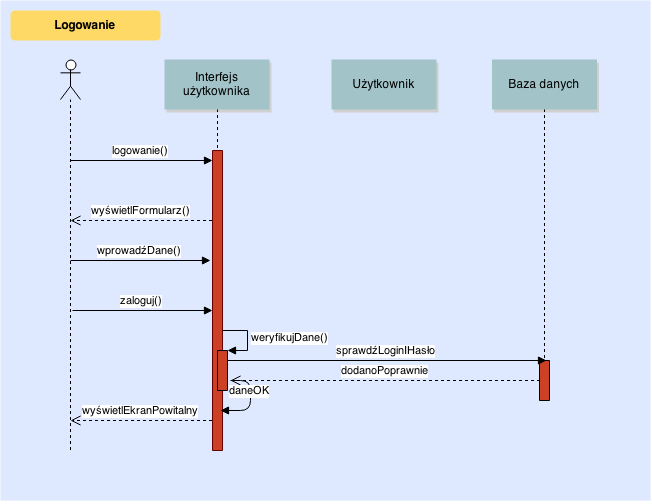
\includegraphics[width=\textwidth]{images/logowanie.png}
  \caption{Diagram sekwencji dla przypadku użycia~\ref{par:login}~--~Logowanie do aplikacji (scenariusz główny)}
\end{figure}

\paragraph{Wyświetlanie listy użytkowników\newline}
\label{par:userList}
Korzysta z~\ref{par:login}~--~Logowanie do~aplikacji.\\

\textit{Opis słowny} -- niniejszy przypadek użycia umożliwia użytkownikowi wyświetlenie listy użytkowników
korzystających z~systemu.

\begin{longtable}{|p{5cm}|p{7cm}|}
  \hline \textbf{Aktor} & Użytkownik \\ \hline
  \textbf{Warunki początkowe} & Użytkownik jest zalogowany \\ \hline
  \textbf{Opis przebiegu interakcji} & Wybór strony z~użytkownikami \\ \hline
  \textbf{Sytuacje wyjątkowe} & Użytkownik nie jest zalogowany \\ \hline
  \textbf{Warunki końcowe} & Wyświetlona lista użytkowników \\ \hline
\end{longtable}

\noindent \textit{Scenariusz główny:}
\begin{enumerate}
  \item Użytkownik otwiera stronę ,,Użytkownicy''.
  \item Jeśli użytkownik nie jest zalogowany, aplikacja wymaga zalogowania, inicjując~\ref{par:login}~--~Logowanie do~aplikacji.
  \item Aplikacja wyświetla użytkowników zarejestrowanych w~systemie.
\end{enumerate}

\begin{figure}[H]
  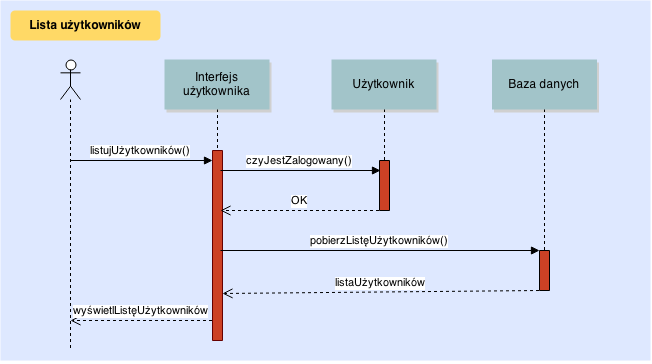
\includegraphics[width=\textwidth]{images/listuj_uzytkownikow.png}
  \caption{Diagram sekwencji dla przypadku użycia~\ref{par:userList}~--~Wyświetlanie listy użytkowników (scenariusz główny)}
\end{figure}

\paragraph{Edycja danych użytkownika\newline}
\label{par:editUser}
Korzysta z~\ref{par:login}~--~Logowanie do~aplikacji.\\

\textit{Opis słowny} -- niniejszy przypadek użycia umożliwia użytkownikowi edycję danych dotyczących jego profilu.

\begin{longtable}{|p{5cm}|p{7cm}|}
  \hline \textbf{Aktor} & Użytkownik \\ \hline
  \textbf{Warunki początkowe} & Użytkownik jest zalogowany \\ \hline
  \textbf{Opis przebiegu interakcji} & Wybór strony z~profilem, wprowadzenie danych, kliknięcie przycisku, zatwierdzenie \\ \hline
  \textbf{Sytuacje wyjątkowe} & Błędnie wprowadzone dane \\ \hline
  \textbf{Warunki końcowe} & Dane użytkownika zaktualizowane w~systemie \\ \hline
\end{longtable}

\noindent \textit{Scenariusz główny:}
\begin{enumerate}
  \item Użytkownik loguje się do aplikacji, tak jak w~scenariuszu~\ref{par:login}~--~Logowanie do aplikacji.
  \item Użytkownik otwiera stronę ,,Profil''.
  \item Użytkownik naciska przycisk ,,Edytuj profil''.
  \item Aplikacja wyświetla okno zawierające dane użytkownika.
  \item Użytkownik edytuje imię, nazwisko, adres e-mail lub hasło i~naciska przycisk ,,Zapisz''.
  \item System prosi użytkownika o~potwierdzenie zmiany poprzez wpisanie starego hasła.
  \item System weryfikuje wprowadzone dane.
  \item Jeżeli dane są prawidłowe, system edytuje dane użytkownika.
\end{enumerate}

\noindent \textit{Scenariusz alternatywny -- niepoprawne dane:}
\begin{enumerate}
  \item[1-7.] Jak w~scenariuszu głównym.
  \item[8.] System wyświetla informacje o~wykrytym błędzie.
  \item[9.] Użytkownik poprawia dane i~naciska przycisk ,,Zapisz''.
  \item[10.] Powrót do kroku 7.~ze scenariusza głównego.
\end{enumerate}

\begin{figure}[H]
  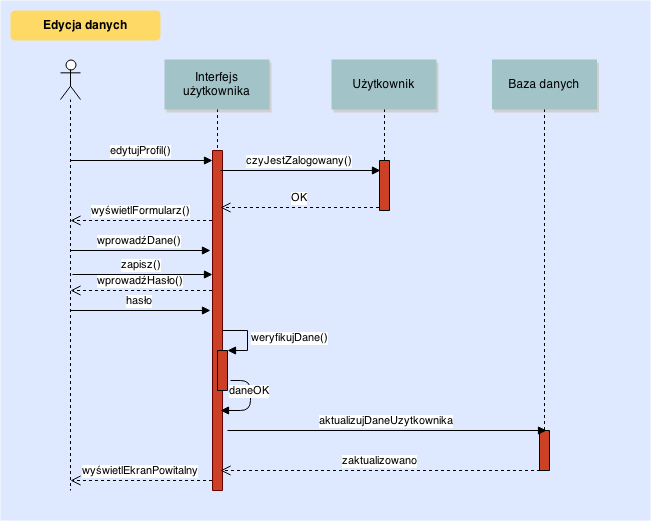
\includegraphics[width=\textwidth]{images/edytuj_uzytkownika.png}
  \caption{Diagram sekwencji dla przypadku użycia~\ref{par:editUser}~--~Edycja danych użytkownika (scenariusz główny)}
\end{figure}

\newpage
\paragraph{Usunięcie użytkownika\newline}
\label{par:deleteUser}
Korzysta z~\ref{par:login}~--~Logowanie do~aplikacji.\\

\textit{Opis słowny} -- niniejszy przypadek użycia umożliwia użytkownikowi skasowanie swojego profilu z~systemu.

\begin{longtable}{|p{5cm}|p{7cm}|}
  \hline \textbf{Aktor} & Użytkownik \\ \hline
  \textbf{Warunki początkowe} & Użytkownik jest zalogowany \\ \hline
  \textbf{Opis przebiegu interakcji} & Wybór strony z~profilem, wprowadzenie danych, kliknięcie przycisku \\ \hline
  \textbf{Sytuacje wyjątkowe} & Błędnie wprowadzone dane \\ \hline
  \textbf{Warunki końcowe} & Skasowanie użytkownika z~systemu i~wylogowanie \\ \hline
\end{longtable}

\noindent \textit{Scenariusz główny:}
\begin{enumerate}
  \item Użytkownik loguje się do aplikacji, tak jak w~scenariuszu~\ref{par:login}~--~Logowanie do aplikacji.
  \item Użytkownik otwiera stronę ,,Profil''.
  \item Użytkownik naciska przycisk ,,Usuń użytkownika''.
  \item System prosi użytkownika o~potwierdzenie decyzji poprzez wpisanie hasła i~naciśnięcie przycisku ,,Usuń''.
  \item System weryfikuje poprawność hasła.
  \item Jeżeli hasło jest zgodne, aplikacja usuwa informacje o~użytkowniku i~następuje wylogowanie.
\end{enumerate}

\noindent \textit{Scenariusz alternatywny -- użytkownik nie potwierdza decyzji:}
\begin{enumerate}
  \item[1-5.] Jak w~scenariuszu głównym.
  \item[6.] Użytkownik nacisnął przycisk ,,Anuluj''.
  \item[7.] System powraca do strony ,,Profil''.
\end{enumerate}

\noindent \textit{Scenariusz alternatywny -- niepoprawne dane:}
\begin{enumerate}
  \item[1-5.] Jak w~scenariuszu głównym.
  \item[6.] System wyświetla informację o~wykrytym błędzie.
  \item[7.] Użytkownik poprawia hasło i~naciska przycisk ,,Usuń''.
  \item[7.] Powrót do kroku 5.~ze scenariusza głównego.
\end{enumerate}

\begin{figure}[H]
  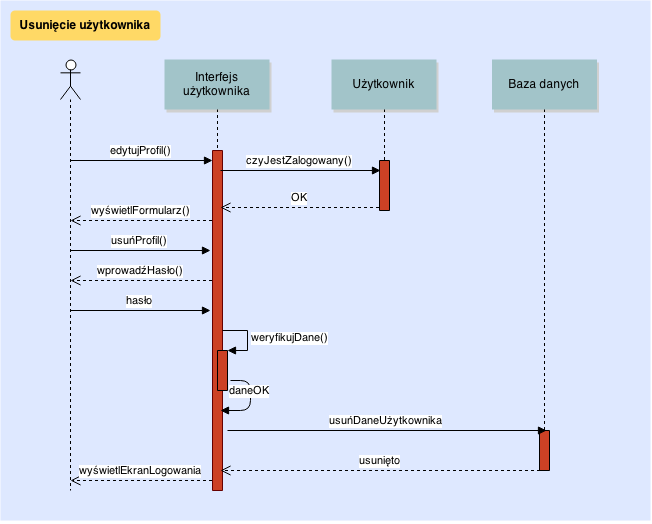
\includegraphics[width=\textwidth]{images/usun_uzytkownika.png}
  \caption{Diagram sekwencji dla przypadku użycia~\ref{par:deleteUser}~--~Usunięcie użytkownika (scenariusz główny)}
\end{figure}

\subsubsection{Opis przypadków użycia -- konta}

\begin{figure}[H]
  \centering
  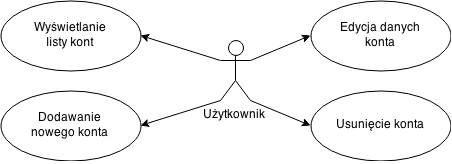
\includegraphics[width=0.9\textwidth]{images/use-cases-accounts.png}
  \caption{Diagram przypadków użycia związanych z~zarządzaniem kontami.}
\end{figure}

\newpage
\paragraph{Wyświetlanie listy kont\newline}
\label{par:accountsView}
Korzysta z~\ref{par:login}~--~Logowanie do~aplikacji.\\
\indent Funkcja generalizująca dla~\ref{par:accountCreate},~\ref{par:accountEdit} oraz~\ref{par:accountDelete}.\\

\textit{Opis słowny} -- niniejszy przypadek użycia umożliwia użytkownikowi wyświetlenie listy kont, które są~do~niego przypisane w~programie. Dzięki temu może on~łatwo nimi zarządzać oraz monitorować ich stan.\\

\begin{tabular}{|l|l|}
  \hline \textbf{Aktor} & Użytkownik \\ \hline
  \textbf{Warunki początkowe} & Użytkownik jest zalogowany \\ \hline
  \textbf{Opis przebiegu interakcji} & Wybór strony z~kontami \\ \hline
  \textbf{Sytuacje wyjątkowe} & Brak \\ \hline
  \textbf{Warunki końcowe} & Wyświetlona lista posiadanych kont \\ \hline
\end{tabular}\\\\

\noindent \textit{Scenariusz główny:}
\begin{enumerate}
  \item Użytkownik otwiera stronę ,,Konta''.
  \item Jeśli użytkownik nie jest zalogowany, aplikacja wymaga zalogowania, inicjując~\ref{par:login}~--~Logowanie do~aplikacji.
  \item Aplikacja wyświetla konta należące do zalogowanego użytkownika.
\end{enumerate}

\begin{figure}[H]
  \centering
  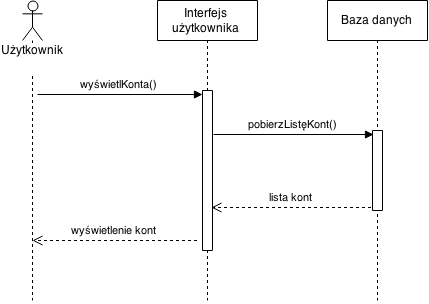
\includegraphics[width=0.7\textwidth]{images/sequence-diagram-accounts-view.png}
  \caption{Diagram sekwencji dla przypadku użycia~\ref{par:accountsView}~--~Wyświetlenie listy kont}
\end{figure}

\paragraph{Utworzenie nowego konta\newline}
\label{par:accountCreate}
Funkcja~specjalizująca~dla~\ref{par:accountsView}~--~Wyświetlanie listy kont.\\

\textit{Opis słowny} -- niniejszy przypadek użycia umożliwia użytkownikowi dodawanie nowych kont. Dzięki temu ma~on możliwość kontrolowania stanu wszystkich posiadanych przez niego fizycznie kont -- np. oszczędnościowych lub walutowych oraz definiowania transakcji pomiędzy nimi.\\

\begin{tabular}{|l|p{9cm}|}
  \hline \textbf{Aktor} & Użytkownik \\ \hline
  \textbf{Warunki początkowe} & Użytkownik jest zalogowany \\ \hline
  \textbf{Opis przebiegu interakcji} & Wybór strony z~kontami, kliknięcie przycisku, wprowadzenie danych oraz zatwierdzenie \\ \hline
  \textbf{Sytuacje wyjątkowe} & Niepoprawne dane \\ \hline
  \textbf{Warunki końcowe} & Nowe konto dodane do systemu \\ \hline
\end{tabular}\\\\

\noindent \textit{Scenariusz główny:}
\begin{enumerate}
  \item[1-3.] Jak w~funkcji generalizującej~\ref{par:accountsView}~--~Wyświetlanie listy kont.
  \item[4.] Użytkownik klika przycisk ,,Dodaj nowe konto''.
  \item[5.] Aplikacja wyświetla okno zawierające pola z~danymi dla nowego konta.
  \item[6.] Użytkownik wprowadza nazwę konta, początkowe saldo, wybiera walutę, typ konta i~klika przycisk ,,Dodaj''.
  \item[7.] System weryfikuje wprowadzone dane (np. czy para użytkownik-nazwa jest unikatowa).
  \item[8.] Jeśli dane są~prawidłowe, system tworzy nowe konto i~powiadamia o~tym użytkownika.
\end{enumerate}

\noindent \textit{Scenariusz alternatywny -- niepoprawne dane:}
\begin{enumerate}
  \item[1-7.] Jak w~scenariuszu głównym.
  \item[8.] System wyświetla informację o wykrytym błędzie.
  \item[9.] Użytkownik poprawia dane i~wciska przycisk ,,Dodaj''.
  \item[10.] Powrót do kroku 7 ze~scenariusza głównego.
\end{enumerate}

\begin{figure}[H]
  \centering
  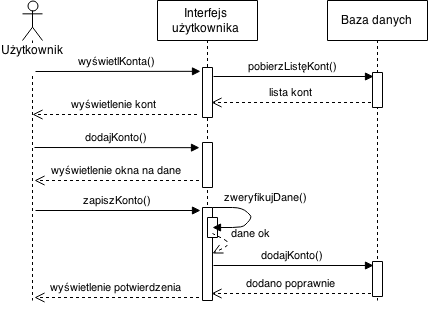
\includegraphics[width=0.7\textwidth]{images/sequence-diagram-account-create.png}
  \caption{Diagram sekwencji dla przypadku użycia~\ref{par:accountCreate}~--~Utworzenie nowego konta}
\end{figure}

\paragraph{Edycja danych konta\newline}
\label{par:accountEdit}
Funkcja~specjalizująca~dla~\ref{par:accountsView}~--~Wyświetlanie listy kont.\\

\textit{Opis słowny} -- niniejszy przypadek użycia umożliwia użytkownikowi edycję danych konta. Dzięki temu ma~on możliwość aktualizowania danych oraz zapewnienia ich zgodności ze~stanem faktycznym -- poza systemem.\\

\begin{tabular}{|l|p{9cm}|}
  \hline \textbf{Aktor} & Użytkownik \\ \hline
  \textbf{Warunki początkowe} & Użytkownik jest zalogowany i~posiada przynajmniej jedno konto \\ \hline
  \textbf{Opis przebiegu interakcji} & Wybór strony z~kontami, wybór konta, kliknięcie przycisku, wprowadzenie danych oraz zatwierdzenie \\ \hline
  \textbf{Sytuacje wyjątkowe} & Niepoprawne dane \\ \hline
  \textbf{Warunki końcowe} & Edycja danych konta w~systemie \\ \hline
\end{tabular}\\\\

\noindent \textit{Scenariusz główny:}
\begin{enumerate}
  \item[1-3.] Jak w~funkcji generalizującej~\ref{par:accountsView}~--~Wyświetlanie listy kont.
  \item[4.] Użytkownik zaznacza jedno z~kont i~klika przycisk ,,Edytuj'' obok niego.
  \item[5.] Aplikacja wyświetla okno zawierające dane zaznaczonego konta.
  \item[6.] Użytkownik edytuje nazwę konta, walutę lub typ konta i~klika przycisk ,,Zapisz''.
  \item[7.] System weryfikuje wprowadzone dane (np. czy para użytkownik-nazwa jest unikatowa).
  \item[8.] Jeśli dane są~prawidłowe, system edytuje konto i~powiadamia o~tym użytkownika.
\end{enumerate}

\noindent \textit{Scenariusz alternatywny -- niepoprawne dane:}
\begin{enumerate}
  \item[1-7.] Jak w~scenariuszu głównym.
  \item[8.] System wyświetla informację o wykrytym błędzie.
  \item[9.] Użytkownik poprawia dane i~wciska przycisk ,,Zapisz''.
  \item[10.] Powrót do kroku 7 ze~scenariusza głównego.
\end{enumerate}

\begin{figure}[H]
  \centering
  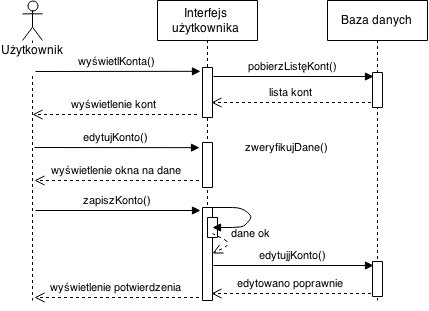
\includegraphics[width=0.7\textwidth]{images/sequence-diagram-account-edit.png}
  \caption{Diagram sekwencji dla przypadku użycia~\ref{par:accountEdit}~--~Edycja danych konta}
\end{figure}

\paragraph{Usunięcie konta\newline}
\label{par:accountDelete}
Funkcja~specjalizująca~dla~\ref{par:accountsView}~--~Wyświetlanie listy kont.\\

\textit{Opis słowny} -- niniejszy przypadek użycia umożliwia użytkownikowi usunięcie konta. Dzięki temu ma~on możliwość ukrycia w~systemie kont już nieużywanych lub nieaktywnych.\\

\begin{tabular}{|l|p{9cm}|}
  \hline \textbf{Aktor} & Użytkownik \\ \hline
  \textbf{Warunki początkowe} & Użytkownik jest zalogowany i~posiada przynajmniej jedno konto \\ \hline
  \textbf{Opis przebiegu interakcji} & Wybór strony z~kontami, wybór konta, kliknięcie przycisku oraz zatwierdzenie \\ \hline
  \textbf{Sytuacje wyjątkowe} & Anulowanie akcji \\ \hline
  \textbf{Warunki końcowe} & Usunięcie konta z~systemu \\ \hline
\end{tabular}\\\\

\noindent \textit{Scenariusz główny:}
\begin{enumerate}
  \item[1-3.] Jak w~funkcji generalizującej~\ref{par:accountsView}~--~Wyświetlanie listy kont.
  \item[4.] Użytkownik zaznacza jedno z~kont i~klika przycisk ,,Usuń'' obok niego.
  \item[5.] Aplikacja wyświetla okno potwierdzenia.
  \item[6.] Użytkownik klika przycisk ,,Usuń'' w~wyświetlonym oknie.
  \item[7.] Aplikacja zamyka okno, usuwa konto i~odświeża listę kont.
\end{enumerate}

\noindent \textit{Scenariusz alternatywny -- przerwanie operacji przez użytkownika:}
\begin{enumerate}
  \item[1-5.] Jak w~scenariuszu głównym.
  \item[6.] Użytkownik wciska przycisk ,,Anuluj''.
  \item[7.] Aplikacja zamyka okno.
\end{enumerate}

\begin{figure}[H]
  \centering
  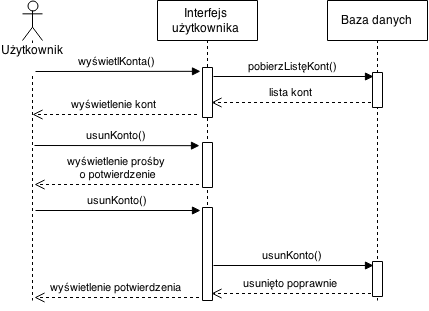
\includegraphics[width=0.7\textwidth]{images/sequence-diagram-account-delete.png}
  \caption{Diagram sekwencji dla przypadku użycia~\ref{par:accountDelete}~--~Usunięcie konta}
\end{figure}

\subsubsection{Opis przypadków użycia -- transakcje}

\begin{figure}[H]
  \centering
  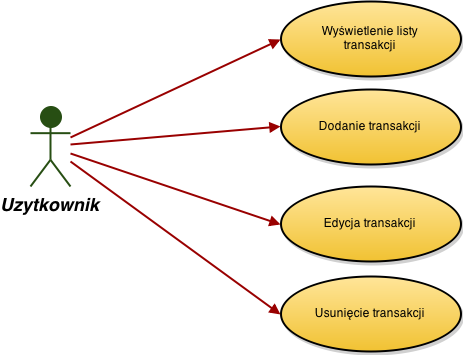
\includegraphics[width=0.9\textwidth]{images/transactions_use_cases.png}
  \caption{Diagram przypadków użycia związanych z~zarządzaniem transakcjami.}
\end{figure}

\paragraph{Wyświetlanie listy transakcji\newline}
\label{par:transactionsView}
Wykorzystuje~\ref{par:login}~--~Logowanie do~aplikacji.\\
\indent Funkcja generalizująca dla~\ref{par:transactionCreate},~\ref{par:transactionEdit} oraz~\ref{par:transactionDelete}.\\

\textit{Opis słowny} -- użytkownik będzie chciał wyświetlić listę transakcji zarejestrowanych w~systemie. Oprócz zwykłej listy zebranych danych, potrzebna jest możliwość filtrowania, co~ułatwi użytkownikowi przeglądanie listy.

\begin{longtable}{|p{5cm}|p{7cm}|}
  \hline \textbf{Aktor} & Użytkownik \\
  \hline \textbf{Warunki początkowe} & Użytkownik jest zalogowany \\
  \hline \textbf{Opis przebiegu interakcji} & Wybór strony z~transakcjami, wprowadzenie parametrów filtrowania \\
  \hline \textbf{Sytuacje wyjątkowe} & Żądanie filtrowania danych \\
  \hline \textbf{Warunki końcowe} & Wyświetlona lista żądanych transakcji \\
  \hline
\end{longtable}

\noindent \textit{Scenariusz główny:}
\begin{enumerate}
  \item Użytkownik otwiera stronę ,,Transakcje''.
  \item Jeśli użytkownik nie jest zalogowany, aplikacja wymaga zalogowania, inicjując~\ref{par:login}~--~Logowanie do~aplikacji.
  \item Aplikacja wyświetla listę transakcji powiązanych z~kontem danego użytkownika.
\end{enumerate}

\noindent \textit{Scenariusz alternatywny -- filtrowanie transakcji:}
\begin{enumerate}
  \item[1-3.] Jak w~scenariuszu głównym.
  \item[4.] Użytkownik wprowadza parametry filtrowania jak nazwa użytkownika, kategoria albo data transakcji.
  \item[5.] Aplikacja odświeża listę transakcji, wyświetlając tylko te, które pasują do podanych filtrów.
\end{enumerate}

\begin{figure}[H]
  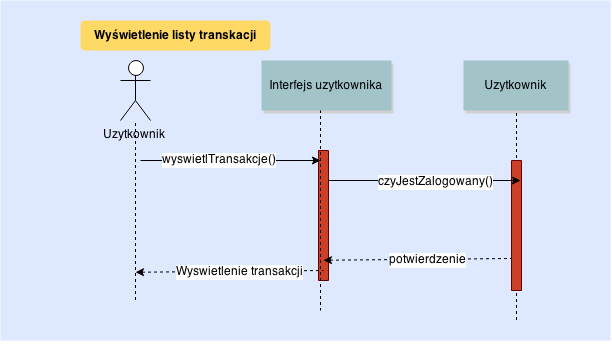
\includegraphics[width=\textwidth]{images/wyswietl_transakcje.png}
  \caption{Diagram sekwencji dla przypadku użycia~\ref{par:transactionsView}~--~Wyświetlenie listy transakcji (scenariusz główny)}
\end{figure}

\paragraph{Utworzenie nowej transakcji\newline}
\label{par:transactionCreate}
Funkcja~specjalizująca~dla~\ref{par:transactionsView}~--~Wyświetlanie listy transakcji.\\

\textit{Opis słowny} -- jedna z~podstawowych funkcjonalności systemu to~dodawanie transakcji, których koszty będą sumowane i~nadzorowane. Akcje te~mają miejsce, gdy użytkownik chce dodać wydatek do systemu.

\begin{longtable}{|p{5cm}|p{7cm}|}
  \hline \textbf{Aktor} & Użytkownik \\
  \hline \textbf{Warunki początkowe} & Użytkownik jest zalogowany oraz posiada przynajmniej jedno konto \\
  \hline \textbf{Opis przebiegu interakcji} & Wybór strony z~transakcjami i~wciśnięcie dodaj, uzupełnienie danych i~zapisanie \\
  \hline \textbf{Sytuacje wyjątkowe} & Wprowadzenie niepoprawnych danych \\
  \hline \textbf{Warunki końcowe} & Dodanie nowej transakcji \\
  \hline
\end{longtable}

\noindent \textit{Scenariusz główny:}
\begin{enumerate}
  \item[1-3.] Jak w~scenariuszu generalizującym~\ref{par:transactionsView}~--~Wyświetlenie listy transakcji.
  \item[4.] Użytkownik wciska przycisk ,,Dodaj transakcję''.
  \item[5.] Aplikacja wyświetla okno z~polami do~wprowadzania danych dotyczących transakcji.
  \item[6.] Użytkownik wprowadza rodzaj transakcji (wpływ/wydatek/transfer), konto od/do, wprowadza wartość, datę, opis i~klika przycisk ,,Dodaj''.
  \item[7.] System weryfikuje wprowadzone dane (np. czy na danym koncie znajduje się wystarczająca ilość pieniędzy).
  \item[8.] Jeśli dane są poprawne, system tworzy nową transakcję, przelicza ilość pieniędzy pozostałych na~koncie i~informuje użytkownika.
\end{enumerate}

\noindent \textit{Scenariusz alternatywny -- niepoprawne dane:}
\begin{enumerate}
  \item[1-7.] Jak w~scenariuszu głównym.
  \item[8.] System wyświetla informację o~wykrytym błędzie.
  \item[9.] Użytkownik poprawia dane i~wciska przycisk ,,Dodaj''.
  \item[10.] Powrót do kroku 7 ze~scenariusza głównego.
\end{enumerate}

\begin{figure}[H]
  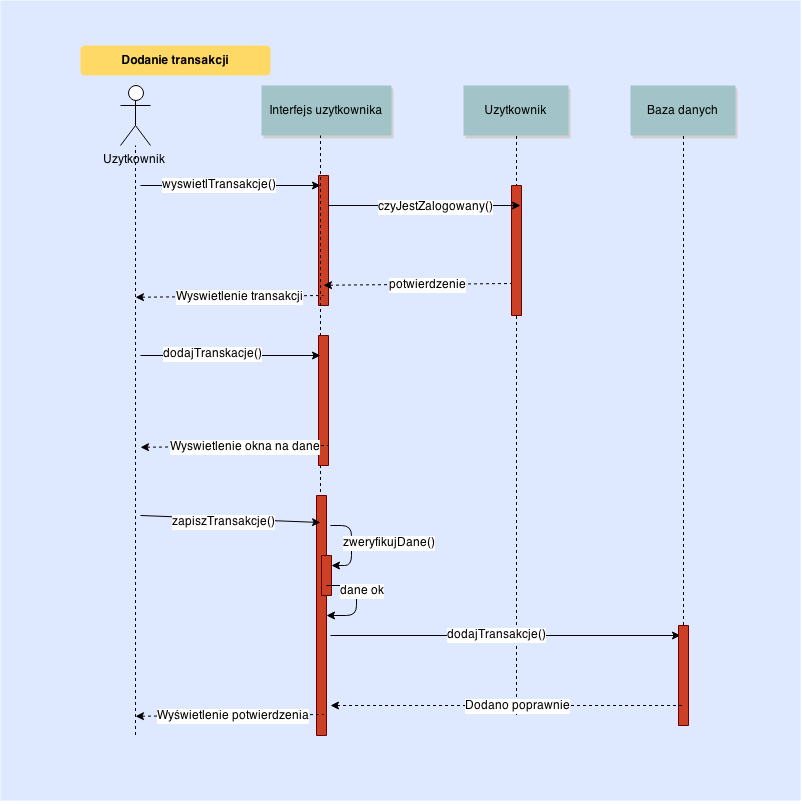
\includegraphics[width=\textwidth]{images/dodanie_transakcji.png}
  \caption{Diagram sekwencji dla przypadku użycia~\ref{par:transactionCreate}~--~Utworzenie nowej transakcji (scenariusz główny)}
\end{figure}

\paragraph{Edycja transakcji\newline}
\label{par:transactionEdit}
Funkcja~specjalizująca~dla~\ref{par:transactionsView}~--~Wyświetlanie listy transakcji.\\

\textit{Opis słowny} -- modyfikacja danych dotyczących wybranej transakcji może być przydatna w~sytuacji, gdy użytkownik wprowadzi błędne dane w~kontekście logicznym, ale które będą poprawnie w~sensie formalnym.

\begin{longtable}{|p{5cm}|p{7cm}|}
  \hline \textbf{Aktor} & Użytkownik \\
  \hline \textbf{Warunki początkowe} & Użytkownik jest zalogowany oraz istnieją transakcje w~systemie \\
  \hline \textbf{Opis przebiegu interakcji} & Wybór strony z transakcjami, wybór żądanej transakcji, modyfikacja danych i~zapisanie \\
  \hline \textbf{Sytuacje wyjątkowe} & Wprowadzenie niepoprawnych danych \\
  \hline \textbf{Warunki końcowe} & Dodanie nowej transakcji \\
  \hline
\end{longtable}

\noindent \textit{Scenariusz główny:}
\begin{enumerate}
  \item[1-3.] Jak w~scenariuszu generalizującym~\ref{par:transactionsView}~--~Wyświetlenie listy transakcji.
  \item[4.] Użytkownik wybiera jedną z~transakcji i~wciska przycisk ,,Edytuj''.
  \item[5.] Aplikacja wyświetla okno z~informacjami o~transakcji.
  \item[6.] Użytkownik modyfikuje dane transakcji (wpływ/wydatek/transfer), konto od/do, wprowadza wartość, datę, opis i~klika przycisk ,,Zapisz''.
  \item[7.] System weryfikuje wprowadzone dane (np. czy na danym koncie znajduje się wystarczająca ilość pieniędzy).
  \item[8.] Jeśli dane są~poprawne, system zapisuje transakcję, przelicza ilość pieniędzy pozostałych na~koncie i~informuje użytkownika.
\end{enumerate}

\noindent \textit{Scenariusz alternatywny -- niepoprawne dane:}
\begin{enumerate}
  \item[1-7.] Jak w~scenariuszu głównym.
  \item[8.] System wyświetla informację o~wykrytym błędzie i~czeka na~poprawkę.
  \item[9.] Użytkownik poprawia dane i~wciska przycisk ,,Zapisz''.
  \item[10.] Powrót do~kroku 7 ze~scenariusza głównego.
\end{enumerate}

\begin{figure}[H]
  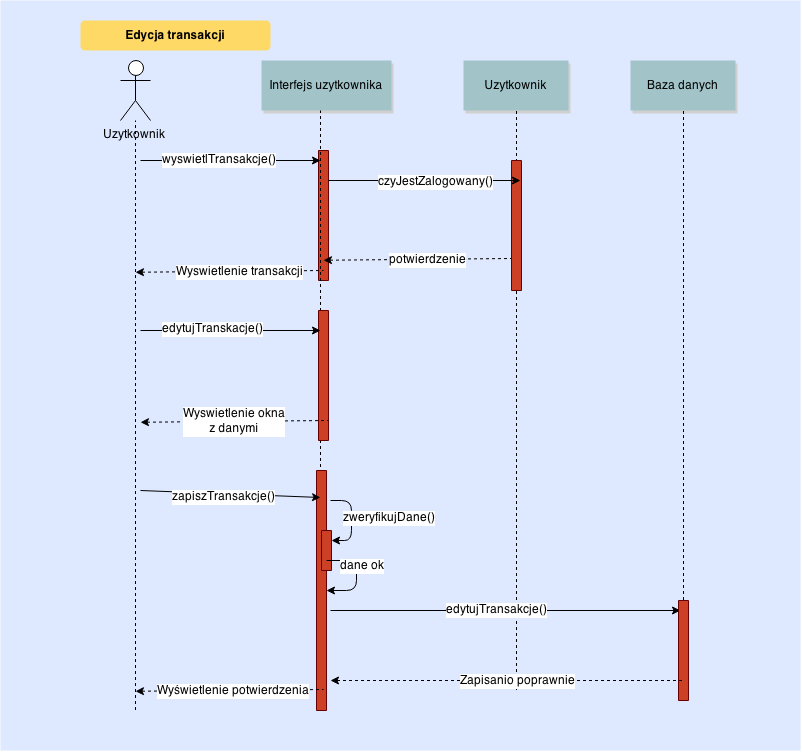
\includegraphics[width=\textwidth]{images/edycja_transakcji.png}
  \caption{Diagram sekwencji dla przypadku użycia~\ref{par:transactionEdit}~--~Edycja transakcji (scenariusz główny)}
\end{figure}

\paragraph{Usuwanie transakcji\newline}
\label{par:transactionDelete}
Funkcja~specjalizująca~dla~\ref{par:transactionsView}~--~Wyświetlanie listy transakcji.\\

\textit{Opis słowny} -- akcje opisane poniżej mają miejsce w~przypadku gdy np. użytkownik zwrócił towar którego dotyczyła transakcja, którą już wprowadził.

\begin{longtable}{|p{5cm}|p{7cm}|}
  \hline \textbf{Aktor} & Użytkownik \\
  \hline \textbf{Warunki początkowe} & Użytkownik jest zalogowany oraz istnieją transakcje w~systemie \\
  \hline \textbf{Opis przebiegu interakcji} & Wybór strony z transakcjami, wybór żądanej transakcji, usunięcie jej \\
  \hline \textbf{Sytuacje wyjątkowe} & Brak \\
  \hline \textbf{Warunki końcowe} & Usunięcie transakcji \\
  \hline
\end{longtable}

\noindent \textit{Scenariusz główny:}
\begin{enumerate}
  \item[1-3.] Jak w~scenariuszu generalizującym~\ref{par:transactionsView}~--~Wyświetlenie listy transakcji.
  \item[4.] Użytkownik wybiera jedną z~transakcji i~wciska przycisk ,,Usuń''.
  \item[5.] Aplikacja wyświetla okienko wymagające potwierdzenia operacji.
  \item[6.] Użytkownik potwierdza operację wciskając przycisk ,,Usuń''.
  \item[7.] Aplikacja zamyka okienko, usuwa transakcję, przelicza ilość pieniędzy na koncie i odświeża listę transakcji.
\end{enumerate}

\noindent \textit{Scenariusz alternatywny -- przerwanie operacji przez użytkownika:}
\begin{enumerate}
  \item[1-5.] Jak w~scenariuszu głównym.
  \item[6.] Użytkownik wciska przycisk ,,Anuluj''.
  \item[7.] Aplikacja zamyka okno.
\end{enumerate}

\begin{figure}[H]
  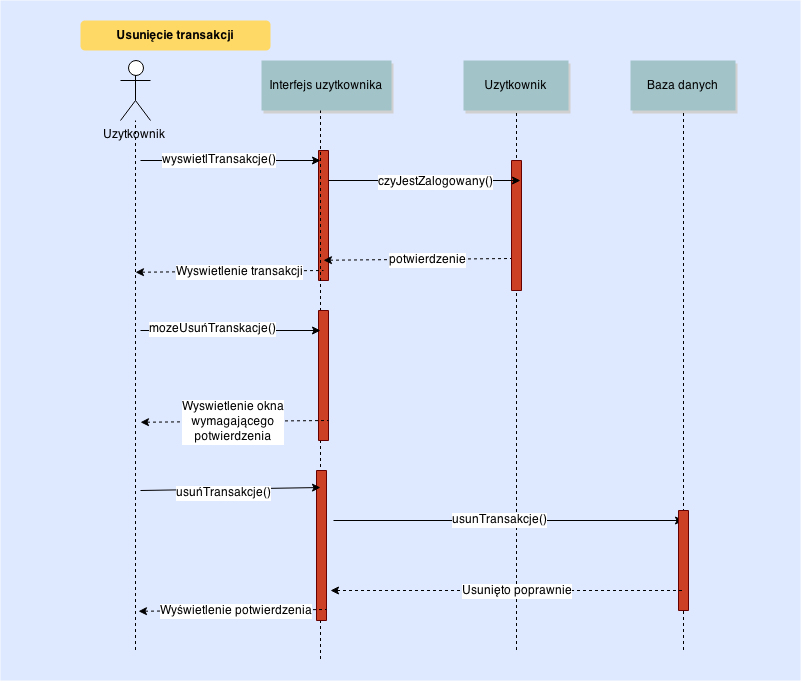
\includegraphics[width=\textwidth]{images/usun_transakcje.png}
  \caption{Diagram sekwencji dla przypadku użycia~\ref{par:transactionDelete}~--~Usuwanie transakcji (scenariusz główny)}
\end{figure}

\subsubsection{Opis przypadków użycia -- budżet}

\begin{figure}[H]
  \centering
  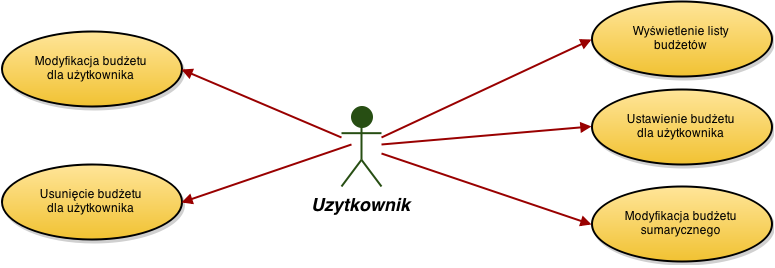
\includegraphics[width=0.9\textwidth]{images/budgets_use_cases.png}
  \caption{Diagram przypadków użycia związanych z~zarządzaniem budżetami.}
\end{figure}

\paragraph{Wyświetlenie budżetów ustawionych w systemie\newline}
\label{par:budgetsList}
Wykorzystuje~\ref{par:login}~--~Logowanie do~aplikacji.\\
\indent Funkcja generalizująca dla~\ref{par:userBudget},~\ref{par:usersBudget},~\ref{par:userBudgetEdit} oraz~\ref{par:userBudgetDelete}.\\

\textit{Opis słowny} -- głównym zadaniem systemu jest nadzorowanie domowego budżetu. Użytkownik będzie chciał przejrzeć aktualny stan budżetów sumarycznych oraz poszczególnych dla każdego z~zarejestrowanych użytkowników.

\begin{longtable}{|p{5cm}|p{7cm}|}
  \hline \textbf{Aktor} & Użytkownik \\
  \hline \textbf{Warunki początkowe} & Użytkownik jest zalogowany \\
  \hline \textbf{Opis przebiegu interakcji} & Wybór strony z budżetami \\
  \hline \textbf{Sytuacje wyjątkowe} & Żądanie filtrowania danych \\
  \hline \textbf{Warunki końcowe} & Wyświetlenie żądanych budżetów \\
  \hline
\end{longtable}

\noindent \textit{Scenariusz główny:}
\begin{enumerate}
  \item Użytkownik otwiera stronę ,,Budżety''.
  \item Jeśli użytkownik nie jest zalogowany, aplikacja wymaga zalogowania, inicjując~\ref{par:login}~--~Logowanie do~aplikacji.
  \item Aplikacja wyświetla budżet sumaryczny dla wszystkich użytkowników oraz listę użytkowników z~budżetami dla każdego z~nich.
\end{enumerate}

\noindent \textit{Scenariusz alternatywny -- filtrowanie wyników:}
\begin{enumerate}
  \item[1-3.] Jak w~scenariuszu głównym.
  \item[4.] Użytkownik wprowadza nazwę konta, którego budżet ma~zostać wyświetlony i~wciska ,,Enter''.
  \item[5.] Aplikacja odświeża listę budżetów wyświetlając tylko jeden dla podanego użytkownika.
\end{enumerate}

\paragraph{Ustawienie budżetu dla określonego użytkownika\newline}
\label{par:userBudget}
Funkcja~specjalizująca~dla~\ref{par:budgetsList}~--~Wyświetlanie budżetów.\\

\textit{Opis słowny} -- celem lepszej kontroli wydatków, użytkownik może chcieć ustawić limit budżetu dla określonego użytkownika, aby ten nie mógł przekroczyć określonej kwoty.

\begin{longtable}{|p{5cm}|p{7cm}|}
  \hline \textbf{Aktor} & Użytkownik \\
  \hline \textbf{Warunki początkowe} & Użytkownik jest zalogowany \\
  \hline \textbf{Opis przebiegu interakcji} & Wybór strony z budżetami, wprowadzenie wymaganych danych, zapisanie nowego budżetu \\
  \hline \textbf{Sytuacje wyjątkowe} & Błędne wprowadzenie danych, przerwanie operacji \\
  \hline \textbf{Warunki końcowe} & Dodanie nowego limitu dla użytkownika \\
  \hline
\end{longtable}

\noindent \textit{Scenariusz główny:}
\begin{enumerate}
  \item[1-3.] Jak w~scenariuszu generalizującym~\ref{par:budgetsList}~--~Wyświetlenie budżetów występujących w~systemie.
  \item[4.] Użytkownik wciska przycisk ,,Dodaj''.
  \item[5.] Aplikacja wyświetla okno z możliwością wyboru konta i~wprowadzenia nowego budżetu.
  \item[6.] Użytkownik wybiera konto, wprowadza nowy budżet i~wciska przycisk "Dodaj".
  \item[7.] Aplikacja weryfikuje poprawność wprowadzonych danych (np. czy liczba nie jest ujemna).
  \item[8.] Jeśli wartość jest poprawna system zapisuje nową wartość budżetu, zamyka okno i~aktualizuje stronę z~budżetami.
\end{enumerate}

\noindent \textit{Scenariusz alternatywny -- przerwanie operacji przez użytkownika:}
\begin{enumerate}
  \item[1-5.] Jak w~scenariuszu głównym.
  \item[6.] Użytkownik wciska przycisk "Anuluj".
  \item[7.] Aplikacja zamyka okno.
\end{enumerate}

\noindent \textit{Scenariusz alternatywny -- niepoprawne dane:}
\begin{enumerate}
  \item[1-7.] Jak w~scenariuszu głównym.
  \item[8.] System wyświetla informację o~niepoprawnych danych.
  \item[9.] Użytkownik wprowadza nową wartość i~wciska przycisk ,,Dodaj''.
  \item[10.] Powrót do kroku 7 ze~scenariusza głównego.
\end{enumerate}

\begin{figure}[H]
  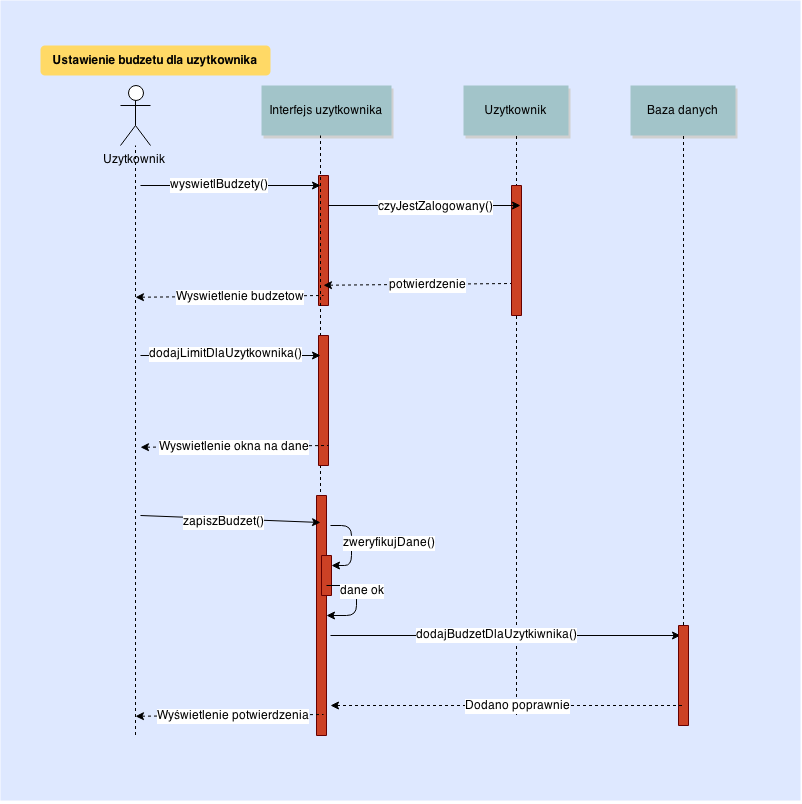
\includegraphics[width=\textwidth]{images/dodanie_budzetu_dla_usera.png}
  \caption{Diagram sekwencji dla przypadku użycia~\ref{par:userBudget}~--~Ustawienie budżetu dla określonego użytkownika (scenariusz główny)}
\end{figure}

\paragraph{Modyfikacja budżetu sumarycznego dla wszystkich użytkowników\newline}
\label{par:usersBudget}
Funkcja~specjalizująca~dla~\ref{par:budgetsList}~--~Wyświetlanie budżetów.\\

\textit{Opis słowny} -- oprócz ustawiania limitu miesięcznego dla danego użytkownika, kluczowym elementem systemu jest modyfikacja limitu sumarycznego dla wszystkich użytkowników danej aplikacji. Wartość ta~musi być zawsze ustawiona, lecz użytkownik może ją~dowolnie modyfikować.

\begin{longtable}{|p{5cm}|p{7cm}|}
  \hline \textbf{Aktor} & Użytkownik \\
  \hline \textbf{Warunki początkowe} & Użytkownik jest zalogowany \\
  \hline \textbf{Opis przebiegu interakcji} & Wybór strony z budżetami, wprowadzenie wymaganych danych, zapisanie budżetu \\
  \hline \textbf{Sytuacje wyjątkowe} & Błędne wprowadzenie danych, przerwanie operacji \\
  \hline \textbf{Warunki końcowe} & Zmodyfikowanie budżetu sumarycznego \\
  \hline
\end{longtable}

\noindent \textit{Scenariusz główny:}
\begin{enumerate}
  \item[1-3.] Jak w~scenariuszu generalizującym~\ref{par:budgetsList}~--~Wyświetlenie budżetów występujących w~systemie.
  \item[4.] Użytkownik wciska przycisk "Edytuj" obok pola wyświetlającego budżet sumaryczny.
  \item[5.] Aplikacja wyświetla okno z~możliwością wprowadzenia nowego budżetu sumarycznego.
  \item[6.] Użytkownik wprowadza nowy budżet i~wciska przycisk ,,Zapisz''.
  \item[7.] Aplikacja weryfikuje poprawność wprowadzonych danych (np. czy liczba nie jest ujemna).
  \item[8.] Jeśli wartość jest poprawna, system zapisuje nową wartość budżetu, zamyka okno i~aktualizuje stronę z budżetami.
\end{enumerate}

\noindent \textit{Scenariusz alternatywny -- przerwanie operacji przez użytkownika:}
\begin{enumerate}
  \item[1-5.] Jak w~scenariuszu głównym.
  \item[6.] Użytkownik wciska przycisk "Anuluj".
  \item[7.] Aplikacja zamyka okno.
\end{enumerate}

\noindent \textit{Scenariusz alternatywny -- niepoprawne dane:}
\begin{enumerate}
  \item[1-7.] Jak w~scenariuszu głównym.
  \item[8.] System wyświetla informację o~niepoprawnych danych.
  \item[9.] Użytkownik wprowadza nową wartość i~wciska przycisk ,,Zapisz''.
  \item[10.] Powrót do kroku 7 ze~scenariusza głównego.
\end{enumerate}

\begin{figure}[H]
  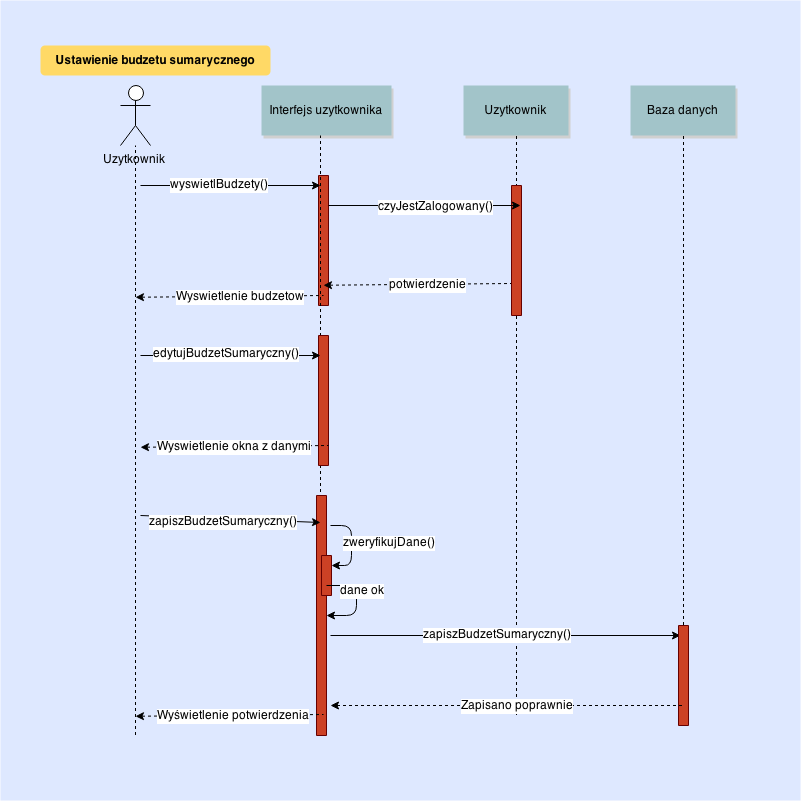
\includegraphics[width=\textwidth]{images/modyfikacja_budzetu_sumarycznego.png}
  \caption{Diagram sekwencji dla przypadku użycia~\ref{par:usersBudget}~--~Ustawienie budżetu sumarycznego (scenariusz główny)}
\end{figure}

\paragraph{Modyfikacja budżetu dla określonego użytkownika\newline}
\label{par:userBudgetEdit}
Funkcja~specjalizująca~dla~\ref{par:budgetsList}~--~Wyświetlanie budżetów.\\

\textit{Opis słowny} -- system musi pozwolić również modyfikować wcześniej ustawiony budżet dla poszczególnych użytkowników, gdyż limity te~mogą się zmieniać np. gdy dziecko dostanie większe kieszonkowe.

\begin{longtable}{|p{5cm}|p{7cm}|}
  \hline \textbf{Aktor} & Użytkownik \\
  \hline \textbf{Warunki początkowe} & Użytkownik jest zalogowany \\
  \hline \textbf{Opis przebiegu interakcji} & Wybór strony z budżetami, wprowadzenie wymaganych danych, zapisanie budżetu \\
  \hline \textbf{Sytuacje wyjątkowe} & Błędne wprowadzenie danych, przerwanie operacji \\
  \hline \textbf{Warunki końcowe} & Zmodyfikowanie budżetu użytkownika \\
  \hline
\end{longtable}

\noindent \textit{Scenariusz główny:}
\begin{enumerate}
  \item[1-3.] Jak w~scenariuszu generalizującym~\ref{par:budgetsList}~--~Wyświetlenie budżetów występujących w~systemie.
  \item[4.] Użytkownik wciska przycisk ,,Edytuj'' obok pola wyświetlającego budżet dla określonego użytkownika.
  \item[5.] Aplikacja wyświetla okno z~możliwością wprowadzenia nowego budżetu.
  \item[6.] Użytkownik wprowadza nowy budżet i~wciska przycisk ,,Zapisz''.
  \item[7.] Aplikacja weryfikuje poprawność wprowadzonych danych (np. czy liczba nie jest ujemna).
  \item[8.] Jeśli wartość jest poprawna, system zapisuje nową wartość budżetu, zamyka okno i~aktualizuje stronę z~budżetami.
\end{enumerate}

\noindent \textit{Scenariusz alternatywny -- przerwanie operacji przez użytkownika:}
\begin{enumerate}
  \item[1-5.] Jak w~scenariuszu głównym.
  \item[6.] Użytkownik wciska przycisk ,,Anuluj''.
  \item[7.] Aplikacja zamyka okno.
\end{enumerate}

\noindent \textit{Scenariusz alternatywny -- niepoprawne dane:}
\begin{enumerate}
  \item[1-7.] Jak w~scenariuszu głównym.
  \item[8.] System wyświetla informację o~niepoprawnych danych.
  \item[9.] Użytkownik wprowadza nową wartość i~wciska przycisk ,,Zapisz''.
  \item[10.] Powrót do kroku 7 ze~scenariusza głównego.
\end{enumerate}

\begin{figure}[H]
  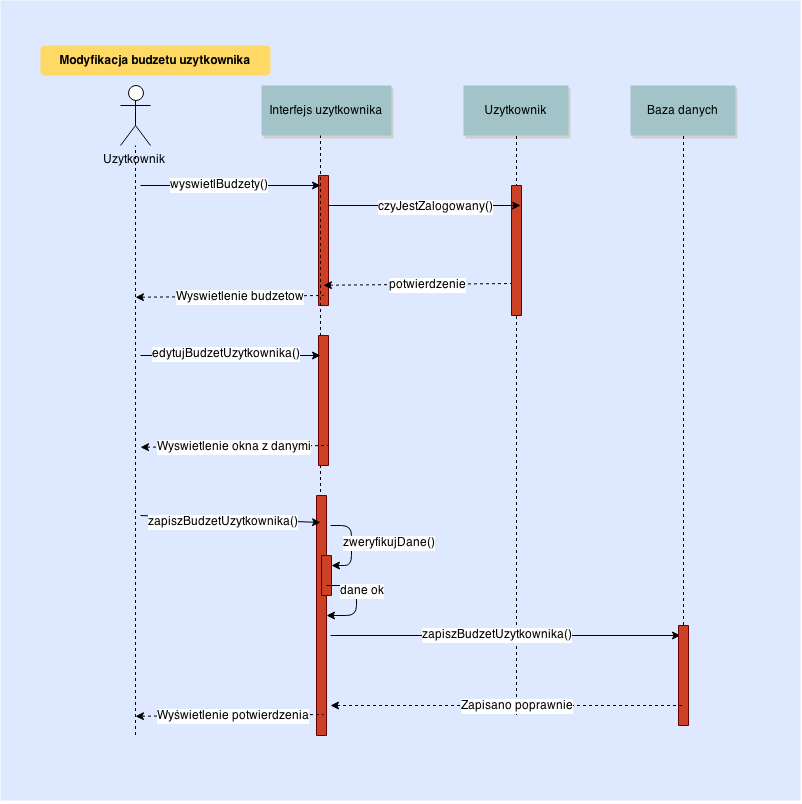
\includegraphics[width=\textwidth]{images/modyfikacja_budzetu_uzytkownika.png}
  \caption{Diagram sekwencji dla przypadku użycia~\ref{par:userBudgetEdit}~--~Modyfikacja budżetu dla określonego użytkownika (scenariusz główny)}
\end{figure}

\paragraph{Usunięcie budżetu dla określonego użytkownika\newline}
\label{par:userBudgetDelete}
Funkcja~specjalizująca~dla~\ref{par:budgetsList}~--~Wyświetlanie budżetów.\\

\textit{Opis słowny} -- akcje te~będą wykonane, gdy np. użytkownik nie będzie dłużej korzystał z~podanej aplikacji lub limit miesięczny przestał go~dotyczyć. Poza tym, polityka ustalania budżetów może ulec zmianie -- na~przykład zamiast ustawiania budżetów na~poszczególne osoby, zacznie obowiązywać tylko budżet sumaryczny.

\begin{longtable}{|p{5cm}|p{7cm}|}
  \hline \textbf{Aktor} & Użytkownik \\
  \hline \textbf{Warunki początkowe} & Użytkownik jest zalogowany oraz istnieje limit ustawiony na~użytkownika \\
  \hline \textbf{Opis przebiegu interakcji} & Wybór strony z budżetami, usunięcie wybranego budżetu \\
  \hline \textbf{Sytuacje wyjątkowe} & Przerwanie operacji \\
  \hline \textbf{Warunki końcowe} & Usunięcie budżetu użytkownika \\
  \hline
\end{longtable}

\noindent \textit{Scenariusz główny:}
\begin{enumerate}
  \item[1-3.] Jak w~scenariuszu generalizującym~\ref{par:budgetsList}~--~Wyświetlenie budżetów występujących w~systemie.
  \item[4.] Użytkownik wciska przycisk ,,Usuń'' obok pola wyświetlającego budżet dla określonego użytkownika.
  \item[5.] Aplikacja wyświetla okno wymagające potwierdzenia operacji.
  \item[6.] Użytkownik potwierdza operację wciskając przycisk ,,Usuń''.
  \item[7.] System usuwa budżet dla określonego użytkownika, zamyka okno i~odświeża stronę z~budżetami.
\end{enumerate}

\noindent \textit{Scenariusz alternatywny -- przerwanie operacji przez użytkownika:}
\begin{enumerate}
  \item[1-5.] Jak w~scenariuszu głównym.
  \item[6.] Użytkownik klika przycisk ,,Anuluj''.
  \item[7.] Aplikacja zamyka okno.
\end{enumerate}

\begin{figure}[H]
  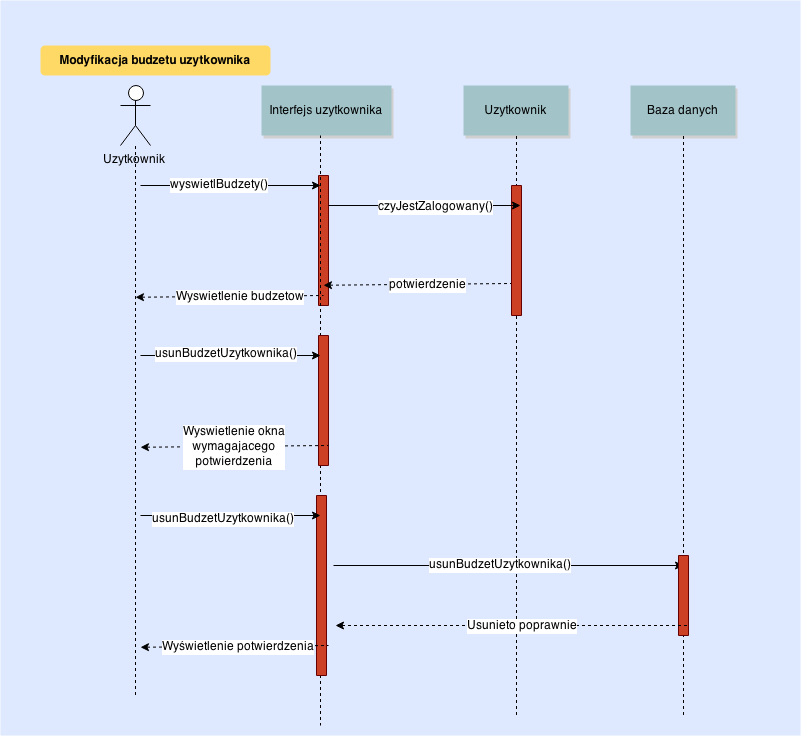
\includegraphics[width=\textwidth]{images/usun_budzet_uzytkownika.png}
  \caption{Diagram sekwencji dla przypadku użycia~\ref{par:userBudgetDelete}~--~Usunięcie budżetu dla określonego użytkownika (scenariusz główny)}
\end{figure}

\subsubsection{Opis przypadków użycia -- raporty}

\begin{figure}[H]
  \centering
  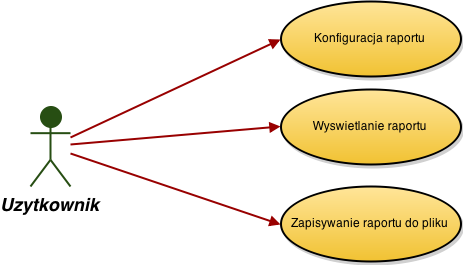
\includegraphics[width=0.7\textwidth]{images/raport_usecases.png}
  \caption{Diagram przypadków użycia związanych z~raportami.}
\end{figure}

\paragraph{Konfiguracja raportu\newline}
\label{par:reportConfig}
Wykorzystuje~\ref{par:login}~--~Logowanie do~aplikacji.\\
\indent Funkcja generalizująca dla~\ref{par:reportView} oraz~\ref{par:reportExport}.\\

\textit{Opis słowny} -- istotną funkcją systemu jest generowanie raportów wizualizujących dane zebrane w~bazie. Użytkownik powinien mieć możliwość określenia budżetów i~zakresu transakcji, których raport ma~dotyczyć.

\begin{longtable}{|p{5cm}|p{7cm}|}
  \hline \textbf{Aktor} & Użytkownik \\
  \hline \textbf{Warunki początkowe} & Użytkownik jest zalogowany \\
  \hline \textbf{Opis przebiegu interakcji} & Wybór opcji raportu \\
  \hline \textbf{Sytuacje wyjątkowe} & Brak \\
  \hline \textbf{Warunki końcowe} & Brak \\
  \hline
\end{longtable}

\noindent \textit{Scenariusz główny:}
\begin{enumerate}
  \item Użytkownik otwiera stronę ,,Raport''.
  \item Jeśli użytkownik nie jest zalogowany, aplikacja wymaga zalogowania, inicjując~\ref{par:login}~--~Logowanie do~aplikacji.
  \item Aplikacja wyświetla pola~do wprowadzania opcji raportu
  \item Użytkownika wprowadza parametry raportu, takie jak zakres uwzględnionych transakcji (budżet sumaryczny/budżet indywidualny/wszystkie transakcje użytkownika), zakres dat, rodzaj raportu (tabela/wykres).
\end{enumerate}

\begin{figure}[H]
  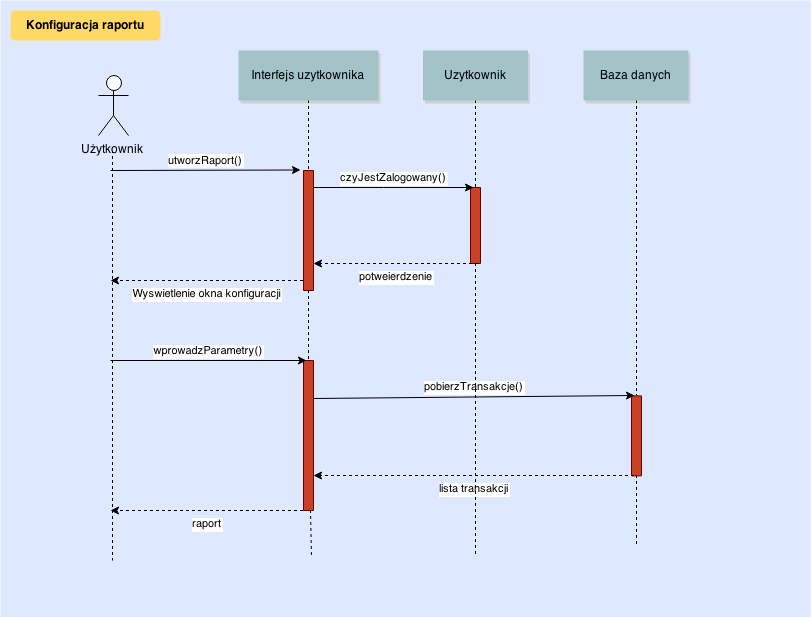
\includegraphics[width=\textwidth]{images/raport_konfig.png}
  \caption{Diagram sekwencji dla przypadku użycia~\ref{par:reportConfig}~--~Konfiguracja raportu (scenariusz główny)}
\end{figure}

\paragraph{Wyświetlanie raportu\newline}
\label{par:reportView}
\indent Funkcja specjalizująca dla~\ref{par:reportConfig}~--~Wyświetlanie konfiguracji raportu.\\

\textit{Opis słowny} -- użytkownik powinien mieć możliwość wyświetlenia raportu w~oknie aplikacji.

\begin{longtable}{|p{5cm}|p{7cm}|}
  \hline \textbf{Aktor} & Użytkownik \\
  \hline \textbf{Warunki początkowe} & Użytkownik jest zalogowany, parametry raportu są~wybrane \\
  \hline \textbf{Opis przebiegu interakcji} & Wyświetlenie raportu \\
  \hline \textbf{Sytuacje wyjątkowe} & Pusty raport \\
  \hline \textbf{Warunki końcowe} & Brak \\
  \hline
\end{longtable}

\noindent \textit{Scenariusz główny:}
\begin{enumerate}
  \item[1-4.] Jak w~scenariuszu generalizującym~\ref{par:reportConfig}~--~Wyświetlanie konfiguracji raportu.
  \item[5.] Użytkownik wciska przycisk ,,Wyświetl raport''.
  \item[6.] Aplikacja wyświetla okno z~raportem w~formie zgodnej z~konfiguracją.
  \item[7.] Użytkownik wciska przycisk ,,Zamknij''.
  \item[8.] Aplikacja zamyka okno.
\end{enumerate}

\noindent \textit{Scenariusz alternatywny~--~brak transakcji w raporcie}
\begin{enumerate}
  \item[1-5.] Jak w~scenariuszu głównym.
  \item[6.] Aplikacja wyświetla informację o~pustym raporcie.
  \item[7.] Powrót do kroku 1. scenariusza głównego.
\end{enumerate}

\begin{figure}[H]
  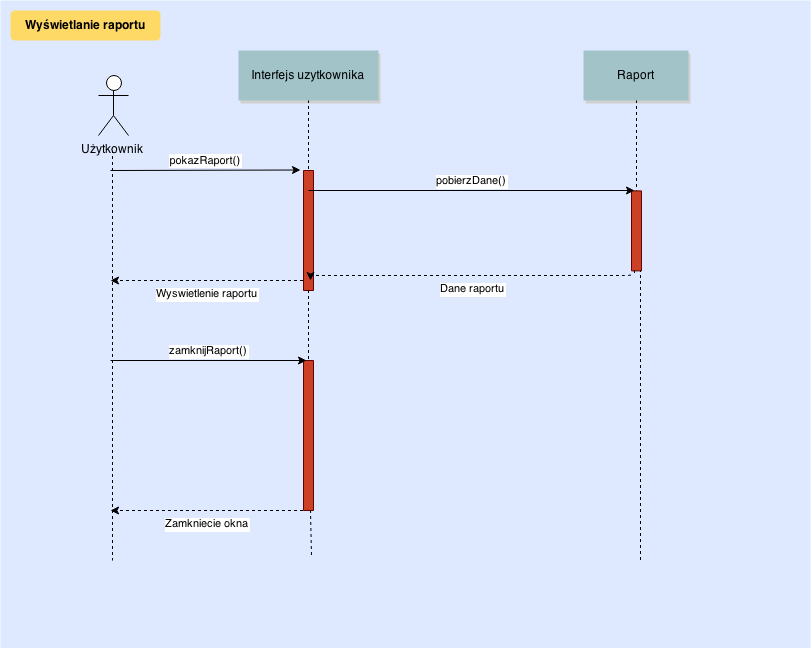
\includegraphics[width=\textwidth]{images/raport_show.png}
  \caption{Diagram sekwencji dla przypadku użycia~\ref{par:reportView}~--~Wyświetlanie raportu (scenariusz główny)}
\end{figure}

\paragraph{Zapisywanie raportu do pliku\newline}
\label{par:reportExport}
\indent Funkcja specjalizująca dla~\ref{par:reportConfig}~--~Wyświetlanie konfiguracji raportu.\\

\textit{Opis słowny} -- aplikacja powinna umożliwiać również zapisanie raportu do~pliku o~określonym formacie.

\begin{longtable}{|p{5cm}|p{7cm}|}
  \hline \textbf{Aktor} & Użytkownik \\
  \hline \textbf{Warunki początkowe} & Użytkownik jest zalogowany, parametry raportu są~wybrane \\
  \hline \textbf{Opis przebiegu interakcji} & Wybór katalogu i~nazwy pliku, zapis raportu \\
  \hline \textbf{Sytuacje wyjątkowe} & Pusty raport, przerwanie operacji \\
  \hline \textbf{Warunki końcowe} & Raport zapisany do pliku \\
  \hline
\end{longtable}

\noindent \noindent \textit{Scenariusz główny:}
\begin{enumerate}
  \item[1-4.] Jak w~scenariuszu generalizującym~\ref{par:reportConfig}~--~Wyświetlanie konfiguracji raportu.
  \item[5.] Użytkownik wciska przycisk ,,Zapisz raport''.
  \item[6.] Aplikacja wyświetla okno wyboru katalogu i~nazwy pliku.
  \item[7.] Użytkownik wybiera katalog i~nazwę pliku i~wciska przycisk ,,Zapisz''.
  \item[8.] Aplikacja zapisuje raport w~odpowiednim formacie do wybranego pliku i~zamyka okno.
\end{enumerate}

\noindent \textit{Scenariusz alternatywny~--~brak transakcji w~raporcie}
\begin{enumerate}
  \item[1-5.] Jak w~scenariuszu głównym.
  \item[6.] Aplikacja wyświetla informację o~pustym raporcie.
  \item[7.] Powrót do kroku 1. scenariusza głównego.
\end{enumerate}

\noindent \textit{Scenariusz alternatywny~--~przerwanie operacji przez użytkownika}
\begin{enumerate}
  \item[1-6.] Jak w~scenariuszu głównym.
  \item[7.] Użytkownik wciska przycisk ,,Anuluj''.
  \item[8.] Aplikacja zamyka okno.
  \item[9.] Powrót do kroku 2. ze scenariusza głównego.
\end{enumerate}

\begin{figure}[H]
  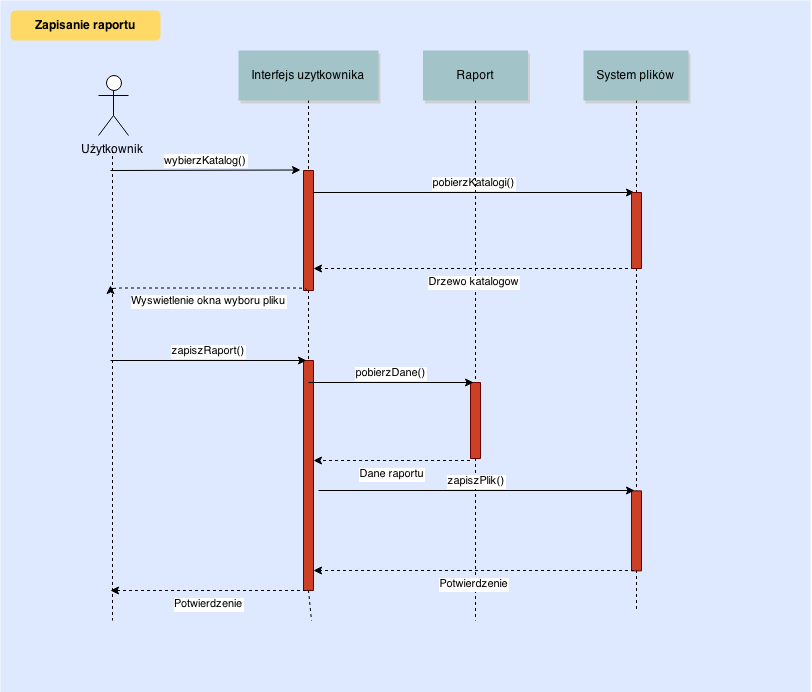
\includegraphics[width=\textwidth]{images/raport_export.png}
  \caption{Diagram sekwencji dla przypadku użycia~\ref{par:reportExport}~--~Zapisywanie raportu do pliku (scenariusz główny)}
\end{figure}

\newpage
\subsection{Wymagania niefunkcjonalne}

\subsubsection{Bezpieczeństwo}

\paragraph{Ograniczenia dostępu\newline}
Priorytet: Wysoki

Złożoność: Niska

Aplikacja nie może pozwalać niezalogowanym użytkownikom na dostęp do danych. Użytkownicy zalogowani mogą mieć dostęp wyłącznie do transakcji własnych oraz transakcji w~budżetach zbiorczych. Ponadto użytkownicy mają możliwość edycji wyłącznie własnych transakcji.

\paragraph{Zabezpieczenie przed nieautoryzowanym odczytem danych\newline}
Priorytet: Wysoki

Złożoność: Średnia

Wszelkie dane przechowywane przez aplikację muszą być zabezpieczone przed odczytem i~modyfikacją bez pośrednictwa aplikacji. Dane nie powinny być przechowywane w~formacie jawnym.

\paragraph{Transakcyjność\newline}
Priorytet: Wysoki

Złożoność: Średnia

Aplikacja nie może pozwalać na realizację niekompletnych operacji. W~wypadku wystąpienia błędu podczas realizacji operacji dane powinny zostać przywrócone do stanu sprzed rozpoczęcia operacji. Nie powinien być możliwy jednoczesny odczyt i~zapis na tych samych danych.

\subsubsection{Użytkowanie}

\paragraph{Wieloinstancyjność\newline}
Priorytet: Średni

Złożoność: Niska

Aplikacja powinna pozwalać wielu użytkownikom na jednoczesne zalogowanie i~korzystanie z~jej funkcji. Nie powinna jednak pozwalać na wiele jednoczesnych sesji tego samego użytkownika.

\subsubsection{Wygląd}

\paragraph{Pomoc kontekstowa\newline}
Priorytet: Niski

Złożoność: Niska

Aplikacja powinna zawierać mechanizm wyświetlania opisów dostępnych opcji wyjaśniających ich przeznaczenie i~zastosowanie.

\newpage
\section{Model analityczny}
Celem niniejszego rozdziału jest zdefiniowanie, jak wyglądać będzie architektura tworzonego systemu. Aby to osiągnąć, w~rozdziale załączone zostały diagramy wykonane zgodnie ze~standardem UML, które stanowią wizualną reprezentację architektury systemu oraz pozwalają na~łatwiejszą analizę stanu projektu.

\subsection{Diagram klas}
Przedstawiony poniżej diagram klas reprezentuje wszystkie wykorzystywane przez Zleceniodawcę elementy składające się na cały system. Diagram ten jest kluczowy przede wszystkim dla deweloperów oraz innych osób zajmujących się bezpośrednio wytwarzaniem oprogramowania, tym niemniej powinien zostać zatwierdzony także przez przedstawicieli Zleceniodawcy -- diagram klas jest bowiem punktem łączącym -- z~jednej strony wyobrażenie klienta o~podziale funkcjonalności, a~z~drugiej decyzje projektowe podjęte przez zespół zajmujący się implementacją.\\

\begin{figure}[H]
  \centering
  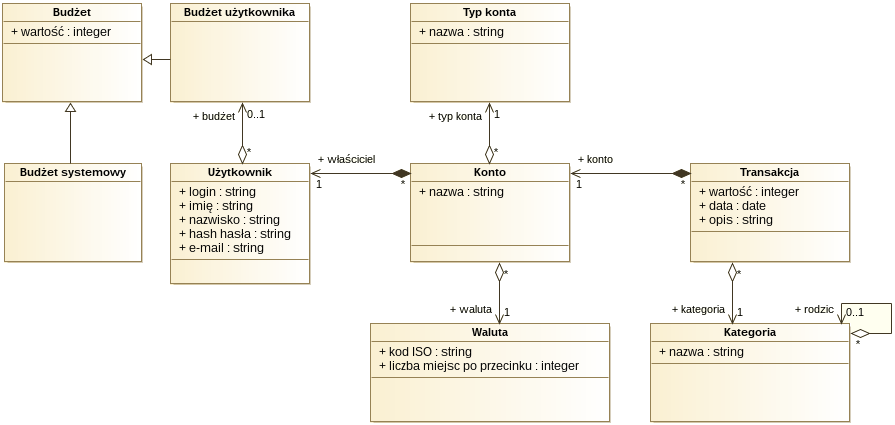
\includegraphics[width=\textwidth]{images/class-diagram.png}
  \caption{Diagram klas systemu.}
\end{figure}

Diagram klas obrazuje zależności (agregacje, kompozycje, relacje dziedziczenia) pomiędzy poszczególnymi klasami na~tyle szczegółowo, by~osoby nieposiadające wykształcenia informatycznego i~nieznające metod programowania obiektowego mogły zrozumieć zasadę podziału bez szczegółowych wyjaśnień. Wszystkie atrybuty czy operacje ważne z~punktu widzenia Zleceniodawcy, które mogą mieć wpływ na~ocenę projektu zostały umieszczone na~diagramie. Poniżej umieszczony został opis każdej z~klas.\\

\textbf{Użytkownik} reprezentuję osobę korzystającą z~aplikacji. Klasa ta~zawiera istotne informacje potrzebne głównie do~uwierzytelniania, takie jak login oraz hash hasła. Pozostałe pola to~na~przykład imię i~nazwisko, czy adres e-mail.\\

\textbf{Konto} jest klasą reprezentującą konto pieniężne (np. oszczędnościowe, osobiste, czy walutowe), które należy do~danego użytkownika. Klasa ta~posiada pola, takie jak nazwa, typ, waluta oraz bieżące saldo.\\

\textbf{Typ konta} jest klasą wydzieloną z~klasy Konto. Utworzenie tej klasy pozwoli na~ograniczenie wartości wprowadzanych w~polu typ konta.\\

\textbf{Waluta} jest kolejną klasą wydzieloną z~klasy Konto. Utworzenie tej klasy pozwoli na~ograniczenie wartości wprowadzanych w~polu waluta. Ponadto przechowuje ona liczbę miejsc po~przecinku, na~jakie zezwala dana waluta, a~więc pozwoli na~walidację wartości pieniężnych wprowadzanych przez użytkownika do~systemu.\\

\textbf{Transakcja} reprezentuje przepływ pieniędzy między kontami. Istnieją trzy typy transakcji -- przychody (pieniądze pochodzące z~konta poza systemem, które trafiają na~jedno z~kont użytkownika), koszty (pieniądze pochodzące z~jednego z~kont użytkownika, które trafiają na~konto poza systemem), lub przelew (pieniądze transferowane pomiędzy dwoma kontami, oba należące do tego samego użytkownika). Klasa ta~zawiera także inne pola, takie jak data, opis (opcjonalnie), czy wartość pieniężna.\\

\textbf{Kategoria} reprezentuje etykiety, które mogą być przypisane do~transakcji. Podobnie jak klasy Waluta oraz Typ konta, jest to~klasa wydzielona z~innej klasy, w~tym przypadku z~Transakcji. Zawiera tylko pole przechowujące nazwę. Kategorie tworzą strukturę drzewa -- jest to~dozwolone poprzez rekurencyjną relację jeden-do-wielu.\\

\textbf{Budżet} jest klasą abstrakcyjną reprezentującą budżet, czyli ograniczenie nakładane na~użytkownika lub cały system. Zawiera ona~tylko jedno pole -- wartość ograniczenia. Istnieją dwie klasy dziedziczące po~klasie Budżet: Budżet użytkownika oraz Budżet systemowy, odpowiednio reprezentują one ograniczenia nałożone na~konkretnego użytkownika, lub cały system.\\

\newpage
\section{Rozwiązania projektowe}

\subsection {Środowisko}
Obecnie coraz większa część systemów informatycznych realizowana jest w~postaci aplikacji z~dostępem z~poziomu przeglądarki internetowej. Taki zabieg pozwala na~bardzo łatwy dostęp do~systemu z~poziomu praktycznie dowolnego urządzenia posiadającego dostęp do~internetu. Innymi kluczowym czynnikiem jest duża łatwość w~dystrybucji takiego rozwiązania i~w~związku z~tym klient również zdecydował się na~zastosowanie takiego podejścia.\\

Środowiskiem pracy dla użytkowników tworzonego systemu będzie przeglądarka internetowa. Dzięki temu klienci będą mogli korzystać z~dostarczonego systemu zarówno przy użyciu komputera osobistego jak i~urządzenia mobilnego. Rozwiązanie takie jak dedykowane aplikacje mogą być przydatne na~niektórych rodzajach urządzeń, jednak tworzenie ich na~wszystkie możliwe rynki (stacjonarne, mobile itp.) stanowiłoby duże wyzwanie i~spowodowało znaczące przekroczenia zarówno budżetu jak i~harmonogramu.\\

Zdecydowano się na~wsparcie następujących rodzajów przeglądarek:
\begin{enumerate}
  \item Google Chrome (od~wersji 23 wzwyż)
  \item Mozilla Firefox (od~wersji 21 wzwyż)
  \item Safari (od~wersji 6 wzwyż)
  \item Opera (od~wersji 15 wzwyż)
  \item Internet Explorer (od~wersji 10 wzwyż)
\end{enumerate}

Pozostałe przeglądarki także powinny poprawnie prezentować stronę internetową sklepu, jednak wsparcie dla nich nie jest wymaganiem, a~co~za~tym idzie, dla przeglądarek tych nie będą przeprowadzane testy.\\

Wygląd strony internetowej powinien być taki sam (z~różnicami maksymalnie 0.04\% zawartości) dla każdej przeglądarki internetowej. Ewentualne różnice wynikające na przykład z~różnicy w~formatach monitorów czy ich wielkości powinny być obsługiwane przez mechanizmy wewnętrzne.\\

Ewentualne aplikacje wspomagające korzystanie ze~sklepu (na~przykład zdobywające coraz większą popularność aplikacje na~urządzenia mobilne) nie znajdują się w~fazie analizy w~niniejszym projekcie, ewentualnie mogą zostać stworzone w~czasie rozbudowy i~utrzymywania systemu. Aby pozostawić możliwość tego rodzaju rozszerzeń należy zadbać o~odpowiedni protokół komunikacyjny uniezależniający działanie serwerów aplikacyjnych i~bazy danych od~klienta, który dostarcza dane i~polecenia.

\subsection{Architektura}
% TODO Kuba

Jedną z~głównych decyzji w~czasie procesu projektowania tworzonego systemu jest wybór odpowiedniej architektury. Nasza
aplikacja będzie wykorzystywała architekturę trójwarstwową (\textit{ang.} three-tier architecture), ponieważ jest to
najpopularniejsza architektura stosowana w~aplikacjach dostępnych z~poziomu przeglądarki internetowej. Architektura
trójwarstwowa jest przykładem aplikacji typu klient-serwer. Dzieli się ją na trzy warstwy, dzięki czemu proces tworzenia
i nanoszenia poprawek jest łatwiejszy. Co więcej, daje to możliwość zredukowania zależności pomiędzy modułami programu.
Architektura składa się z~następujących warstw: 
\begin{itemize}
  \item \textbf{warstwa danych} (\textit{ang.} data tier)~--~odpowiada za trwałe przechowywanie danych, udostępnia
    interfejs do ich pobierania i~modyfikacji. Realizowana za pomocą relacyjnej bazy danych.
  \item \textbf{warstwa logiki biznesowej} (\textit{ang.} business logic tier)~--~odpowiada za logikę całego systemu,
  koordynuje działania odpowiadające operacjom na kontach i~użytkownikach. Znajduje się na serwerze aplikacyjnym. Pełni
  rolę pośrednika pomiędzy pozostałymi warstwami.
  \item \textbf{warstwa prezentacji} (\textit{ang.} presentation tier)~--~odpowiada za prezentowanie aplikacji na
  komputerze użytkownika, zbieranie jego akcji i~przekazywanie ich do warstwy logiki biznesowej.
\end{itemize}

Wybór architektury trójwarstwowej pociąga za sobą technologie w~jakie zostaną zastosowane. Do stworzenia interfejsu
użytkownika wykorzystane zostaną technologie wykorzystywane w~projektowaniu stron internetowych, czyli HTML i~CSS. Aby
poprawić User Experience, można również założyć wykorzystanie języka JavaScript oraz technologii AJAX. Warstwa logiki,
czyli tzw. backend zostanie stworzony przy użyciu języka Java, ze względu na wydajność, łatwość we wprowadzaniu
zmian, oraz rozbudowaną dokumentację. Dodatkowo wykorzystany zostanie framework webowy SpringMVC. Jako system
zarządzania bazą danych (\textit{ang.} DBMS) postanowiono wykorzystać PostgreSQL.

\begin{figure}[H]
  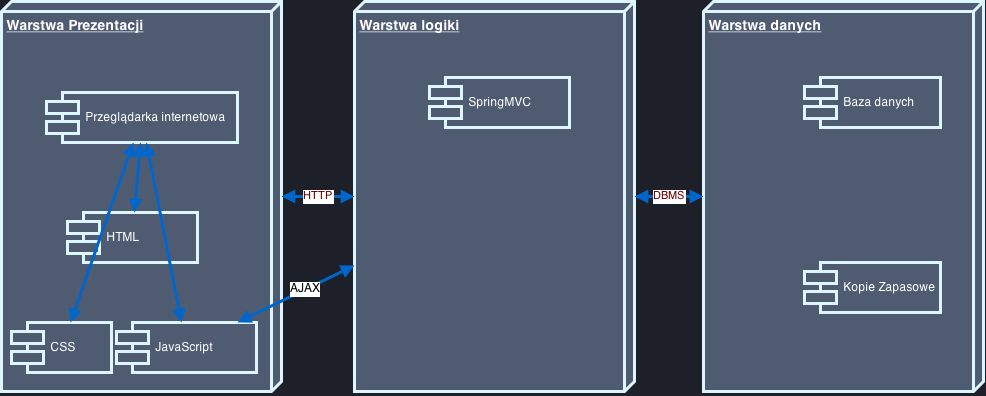
\includegraphics[width=\textwidth]{images/3tier.png}
  \caption{Architektura trójwarstowa, z~zaznaczonymi wybranymi technologiami.}
\end{figure}

\subsection{Sprzęt}

Wdrożenie systemu wymagać będzie zapewnienia odpowiedniej infrastruktury sprzętowej. W celu zapewnienia skalowalności będzie ona podzielona na serwer aplikacyjny i~serwer bazodanowy. Jako że obsługa systemu od strony użytkownika będzie opierać się o~interfejs webowy kompatybilny z!ogromną większością komputerów osobistych wyposażonych w przeglądarkę internetową, wykorzystanie dodatkowych stacji klienckich nie będzie konieczne.

Biorąc pod uwagę takie czynniki jak cena i~wydajność, a~także niezawodność i~głośność pracy, zdecydowano się na wybór komputerów serwerowych z~oferty firmy \textit{Dell}.

\subsubsection{Serwer aplikacyjny}

Jako serwer obsługujący warstwę logiki wybrano \textit{Dell PowerEdge R220} ze względu na korzystny stosunek wydajności do ceny.

\begin{figure}[H]
  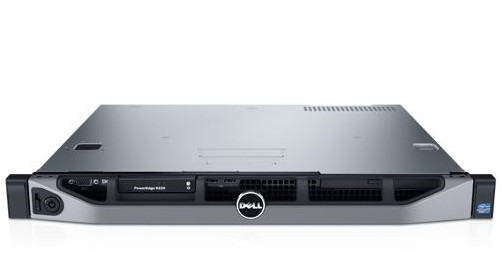
\includegraphics[width=\textwidth]{images/poweredge-r220.jpg}
  \caption{Dell PowerEdge R220}
\end{figure}

\begin{figure}[H]
\begin{center}
\begin{tabular}{|l|l|}
  \hline
  Procesor & Intel® Celeron® G1820 2.7GHz \\ \hline
  Pamięć RAM & 4 x 4GB UDIMM, 1600 MT/s, Low Volt, Single Rank, x8 Data Width \\ \hline
  Dysk & 500GB 7.2k RPM SATA 6Gbps Entry 3.5in Cabled Hard Drive \\ \hline
  Zasilanie & 250W (80+ Silver); auto-ranging (100V--240V) \\ \hline

\end{tabular}
\end{center}
\end{figure}

\subsubsection{Serwer bazy danych}

Baza danych obsługiwana będzie przez serwer \textit{Dell PowerEdge R320}.

\begin{figure}[H]
  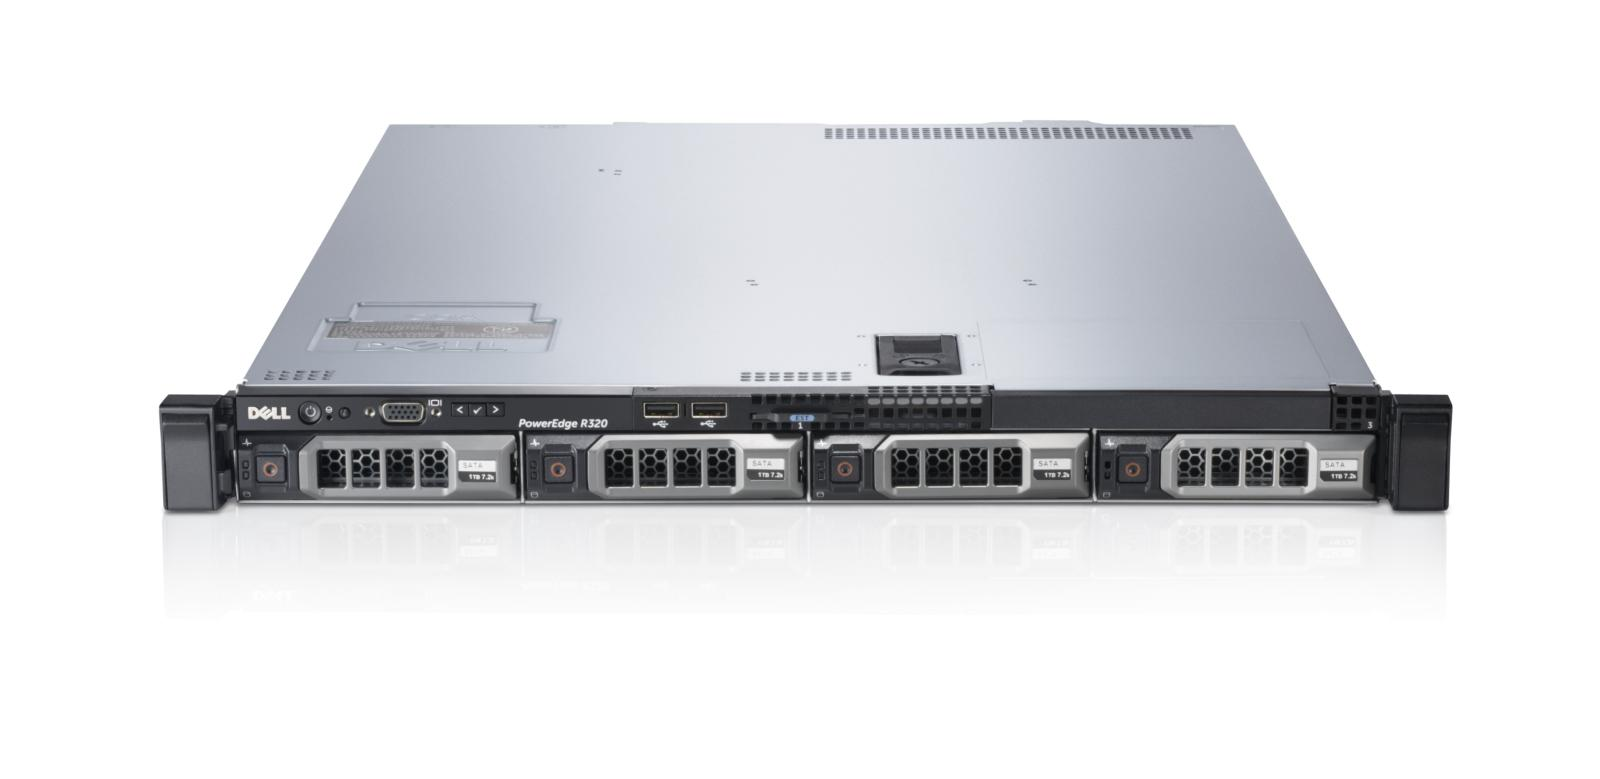
\includegraphics[width=\textwidth]{images/poweredge-r320.jpg}
  \caption{Dell PowerEdge R320}
\end{figure}

\begin{figure}[H]
\begin{center}
\begin{tabular}{|l|l|}
  \hline
  Procesor & Intel® Pentium® 1403 v2 2.60GHz \\ \hline
  Pamięć RAM & 4 x 4GB UDIMM, 1600 MT/s, Low Volt, Single Rank, x8 Data Width \\ \hline
  Dysk & 500GB 7.2k RPM SATA 6Gbps Entry 3.5in Cabled Hard Drive \\ \hline
  Zasilanie & 350W (80+ Silver); auto-ranging (100V--240V) \\ \hline

\end{tabular}
\end{center}
\end{figure}

\subsubsection{Szafa rack}

Oba serwery wyposażone są w obudowy typu \textit{rack 19''} i~są kompatybilne z~wszelkiego rodzaju szafami wykorzystującymi ten standard. Biorąc pod uwagę niewielkie rozmiary i solidność wykonania, sugerowane jest wykorzystanie szafy serwerowej \textit{Signati 12U}.

\begin{figure}[H]
  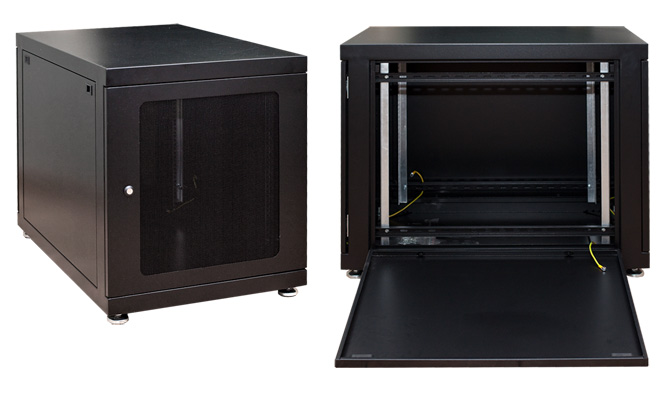
\includegraphics[width=\textwidth]{images/szafa_12U.jpg}
  \caption{Signati 12U}
\end{figure}
%\section{Interfejs użytkownika}

W dzisiejszych czasach interfejs użytkownika graficzny użytkownika stanowi niezwykle istotny element każdego systemu
informatycznego. Powinien on łączyć w~sobie dwie cechy: użyteczność i~atrakcyjność. Ważne jest uzyskanie odpowiedniego
balansu pomiędzy tymi cechami. Skupienie się wyłącznie na użyteczności prawdopodobnie odbije się negatywnie na
atrakcyjności i~odwrotnie. 

Dodatkowo interfejs powinien nawiązywać do aktualnych trendów w~tej dziedzinie. Nawet najładniejsza i~łatwa w~obsłudze
aplikacja, która powstała kilka lat temu nie będzie dorównywała aplikacjom stworzonym na przestrzeni ostatnich miesięcy.
Wynika to głównie ze zmiany podejścia do tworzenia interfejsów. Obecnie projektowane interfejsy muszą często dobrze
przezentować się zarówno na komputerach stacjonarnych, jak i~urządzeniach mobilnych. Wymusza to stosowanie prostych
kontrolek, oraz ograniczanie ilości informacji do niezbędnych dla działania.

Obecny trend wskazuje, że za najładniejsze uznawane są aplikacje minimalistyczne (np.  material design). Przedstawiony
poniżej prototyp interfejsu został stworzony z~myślą o~użyteczności, jednak również jego atrakcyjność można uznać za
nawiązującą do panującej mody.

Należy pamiętać, że jest to jedynie prototyp i~nie prezentuje on wszystkich funkcjonalności, ani widoków jakie będzie
posiadał przyszły system, a~jedynie narzuca pewną konwencje, która powinna zostać zachowana przy tworzeniu pozostałych
elementów.

\newpage

\begin{figure}[H]
  \centering
  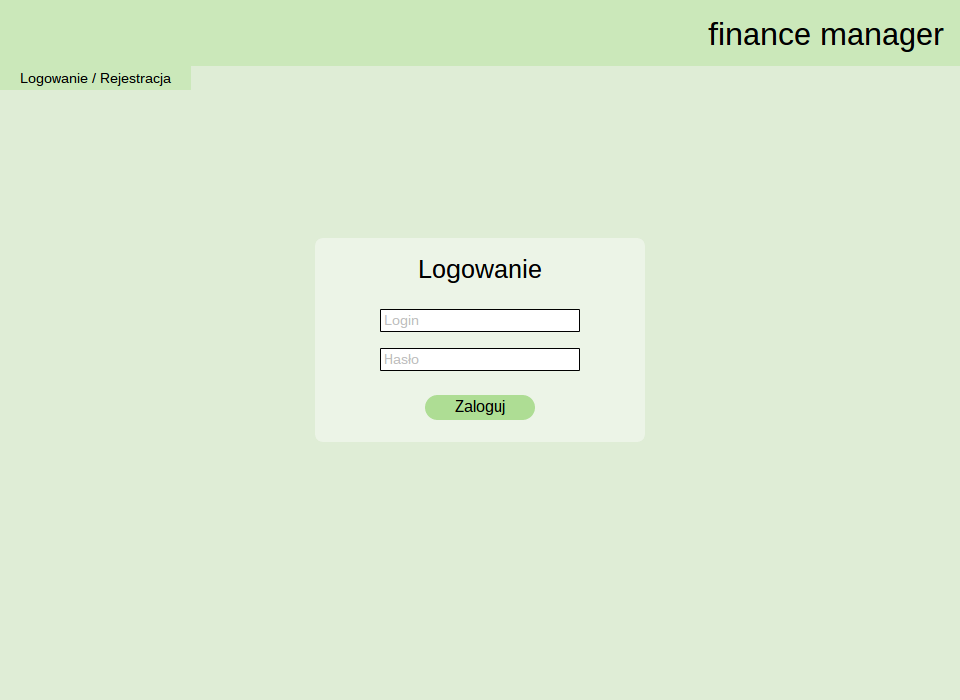
\includegraphics[width=\textwidth]{images/ui-login.png}
  \caption{Prototyp widoku logowania.}
  \label{pic:login}
\end{figure}

Strona startowa jaką zobaczy użytkownik prezentuje się jak na rysunku \ref{pic:login}. Z~tego poziomu każdy użytkownik
posiadający w~systemie konto będzie mógł zalogować się do swojego prywatnego panelu. Jeżeli system odwiedzi użytkownik,
który swojego konta w~systemie nie posiada, będzie on musiał przejść do strony rejestracji, klikając odpowiedni odnośnik
na banerze znajdującym się pod logo aplikacji.


\begin{figure}[H]
  \centering
  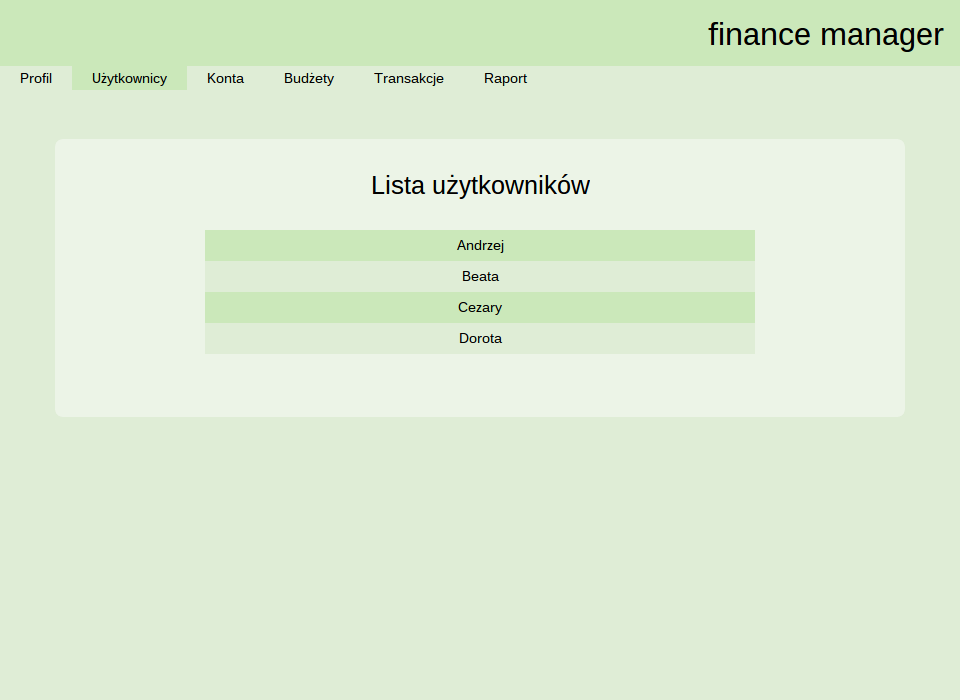
\includegraphics[width=\textwidth]{images/ui-user-list.png}
  \caption{Prototyp widoku z~listą użytkowników.}
  \label{pic:user_list}
\end{figure}

Wszystkie pozostałe prezentowane widoki zakładają, że użytkownik pomyślnie zalogował się do systemu. Na rysunku
\ref{pic:user_list} znajduje się widok z~listą użytkowników, tak aby każdy mógł sprawdzić, kto również posiada konto w
systemie.

\begin{figure}[H]
  \centering
  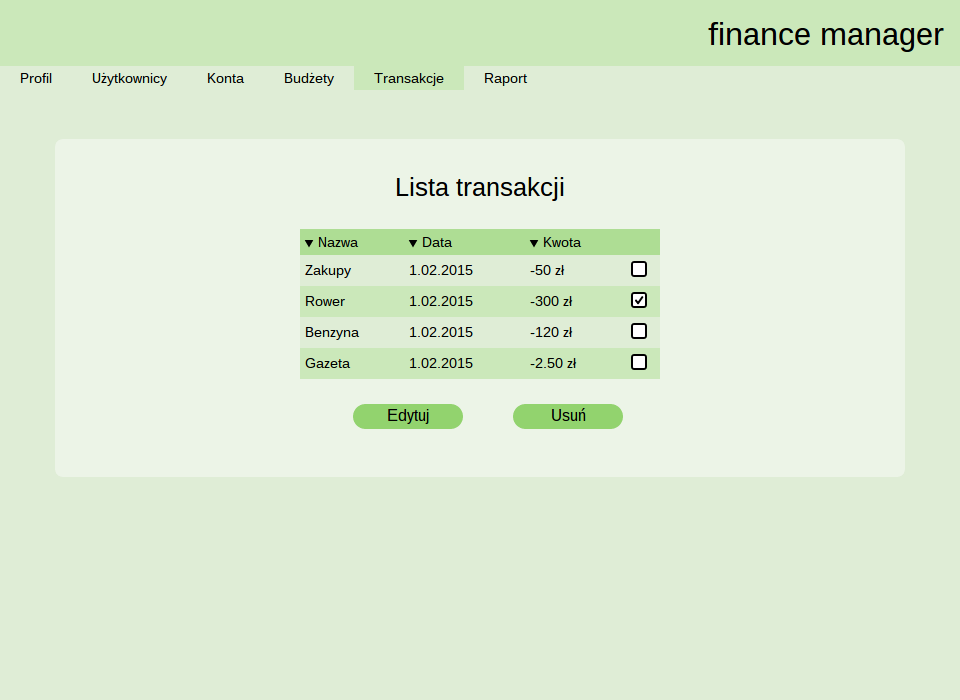
\includegraphics[width=\textwidth]{images/ui-trans.png}
  \caption{Prototyp widoku z~listą transakcji.}
  \label{pic:trans}
\end{figure}

Rysunek \ref{pic:trans} prezentuje widok transakcji. Z~tego poziomu użytkownik może dokonywać przeglądu dokonanych
wydatków, lub uzyskanych przychodów. Po zaznaczeniu odpowiedniej transakcji, uaktywniają się opcje edycji i~usuwania
zaznaczonej transakcji. Dzięki temu można kontrolować przypadkowo wstawione operacje, lub takie które nie mają
znaczącego wpływu na stan konta. Dodakowo, co może się okazać szczególnie przydatne w~przypadku gdy lista transakcji
urośnie do większych rozmiarów, istnieje możliwość sortowania transakcji według jednego z~trzech kluczy.

\begin{figure}[H]
  \centering
  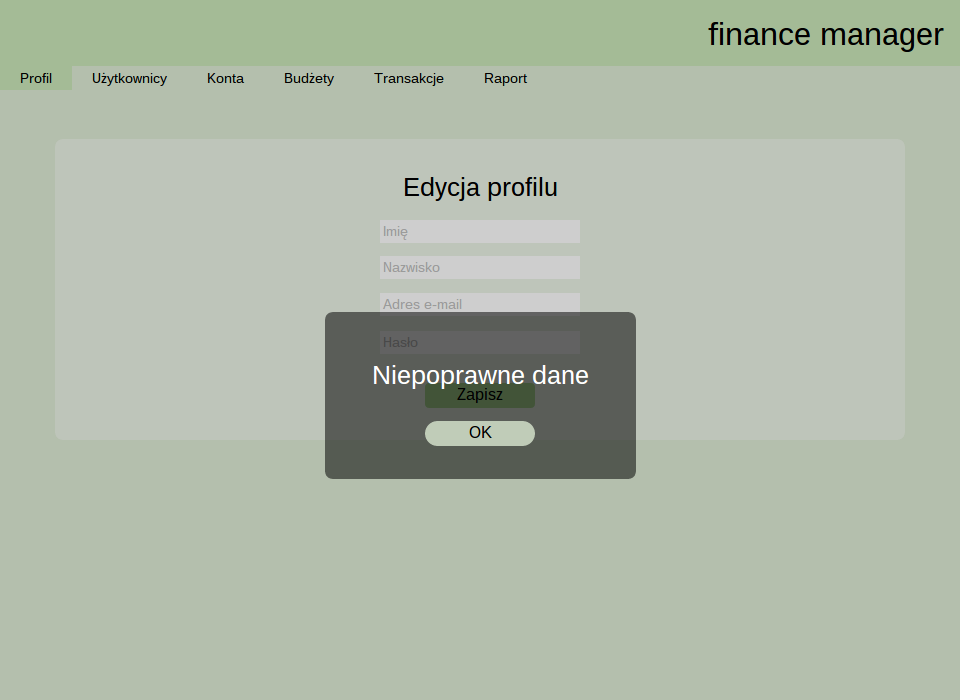
\includegraphics[width=\textwidth]{images/ui-profile-edit-err.png}
  \caption{Prototyp widoku pozwalającego na edycję danych użytkownika, z~wyświetlonym komunikatem o~błędzie.}
  \label{pic:profile_edit}
\end{figure}

Ostatni rysunek  nr \ref{pic:profile_edit} pokazuje widok edycji danych użytkownika. Na pierwszym planie wyświetlony
jest komunikat o~błędzie, aby zaprezentować w~jaki sposób można powiadamiać użytkownika o~występujących problemach.

Pozostałe widoki utworzone zostaną z~zachowaniem wyznaczonych styli i~standardów.


\end{document}
